% Arara build configuration:
% arara: pdflatex: {synctex: on, shell: true}
% arara: bibtex
% nomencl: {style: 'nomencl'}
% pdflatex: { synctex: on }
% pdflatex: { synctex: on }

%\includeonly{chap/legdesign}
\documentclass[listof=totoc,bibliography=totoc,11pt,twoside,BCOR=12mm,DIV=11]{scrbook}
\linespread{1.25}

\renewcommand*{\chapterheadstartvskip}{\vspace*{0cm}}

\renewcommand{\autodot}{}% Remove all end-of-counter dots
\addtokomafont{pagenumber}{\large\sffamily}

%\usepackage{showframe}  %to show typing area, header, footer, margins

\usepackage{microtype} %improve font spacing
\usepackage{parskip}

\usepackage[english]{babel}
\usepackage{amsmath}
\usepackage{amsfonts}
\usepackage{amssymb}
\usepackage[T1]{fontenc}
\usepackage{charter} %set font
%\setkomafont{disposition}{\bfseries}
\addtokomafont{chapter}{\Huge} %set font parameter
\addtokomafont{section}{\huge} %set font parameter
\addtokomafont{subsection}{\LARGE} %set font parameter
\addtokomafont{subsubsection}{\Large} %set font parameter

%\usepackage[headsepline,footsepline]{scrpage2}
%\pagestyle{scrheadings}
%\setheadsepline{3pt}

%\usepackage[round,mcite]{natbib} %bibliography

\usepackage[hidelinks]{hyperref} %hyperlinks in pdf
\usepackage{cleveref}
\crefname{subsection}{subsection}{subsections}

\usepackage{blindtext}  %to create a dummy document
\usepackage{lipsum} %content filler

\usepackage{minted}
\usemintedstyle{fruity}

\usepackage{float}
\usepackage{graphicx}
\DeclareGraphicsExtensions{.pdf,.png,.jpg,.eps} %images without extension
\usepackage{subfig} %use subfigure configurations
%\usepackage{caption}
%\usepackage{subcaption}
\usepackage{epstopdf} %include eps figures
\usepackage[final]{pdfpages} %includepdf
\usepackage[section]{placeins} %no [Htb], place within section
%\usepackage{showframe}

\usepackage{textcomp} %copyright symbols

%Nomenclature
\usepackage[intoc]{nomencl}
\makenomenclature

% customize dictum format:
\setkomafont{dictumtext}{\itshape\small}
\setkomafont{dictumauthor}{\normalfont}
\renewcommand*\dictumwidth{\linewidth}
\renewcommand*\dictumauthorformat[1]{--- #1}
\renewcommand*\dictumrule{}

\begin{document}

\frontmatter
\titlehead{
\begin{center}

\includegraphics[width = 0.35\textwidth]{images/uctround.png}
\end{center}
}
\subject{Faculty of Engineering and the Built Environment \\
Department of Electrical Engineering \\}
\title{{Hopping Control of a Single Leg Robot}}
\subtitle{Prepared for Dr. Amir Patel.
\linebreak
Submitted to the Department of Electrical Engineering\\at the University of Cape Town in partial
fulfilment\\ of the academic requirements\\for a Bachelor of Science (Eng.) degree in Mechatronics.
}
\author{Benjamin Scholtz}
%\date{date}
\publishers{\textbf{Keywords:} robotics, virtual model, compliance control, force control, mechatronics}
\dedication{To all the people that helped me jump!\\ \medskip \includegraphics[width = 0.4\textwidth]{images/leg-mount.png}}
\maketitle
\chapter{Declaration}
\begin{enumerate}
\item I know that plagiarism is wrong. Plagiarism is to use another's work and pretend that it
is one's own.
\item I have used the IEEE convention for citation and referencing. Each contribution to, and
quotation in, this final year project report from the work(s) of other people, has been attributed and has been cited and referenced.
\item This final year project report is my own work.
\item I have not allowed, and will not allow, anyone to copy my work with the intention of passing it off as their own work or part thereof.
\end{enumerate}

\bigskip

\noindent
Name: Benjamin Scholtz \\
Signature: \underline{\hspace{3cm}} \\
Date: \today \\
\chapter{Abstract}

A vertically constrained direct drive robotic leg platform was modelled, simulated, designed, built, and tested in order to better understand rapid acceleration control. The research was performed to investigate the following questions: \textbf{Is a virtual model a suitable replacement for accurate dynamic modelling in complex robotic topologies? Can high fidelity force control be effectively implemented without using force feedback? Is a virtual compliance control system effective in handling high speed impacts and executing rapid acceleration manoeuvres?} The dynamic model of the robot is complex, instead a virtual model uses simulations of components placed on the body of the robot to generate the desired end effector force response. The end effector was virtually modelled in the polar coordinate system as a radial and torsional series spring-damper. The desired virtual model motor torques were generated using the Jacobian kinematic mapping. Proprioceptive force control was possible due to the transparent coupling between the direct drive actuator and end effector. An iterative hardware and software design process was used to enable effective robotic testing - both an embedded communication and control system, and a GUI, were developed for the platform. Experiments were performed in virtual model spring-damping, impact absorption, trajectory tracking, force control, and current control. Jump tests were performed investigating robustness, repeatability, and rapid acceleration control. Force control and virtual model fidelity were verified by critically analysing both theoretical simulated responses and practical data. The robot generated an energy of $3.9\ J/kg$ with a maximum hopping height of $0.4\ m$, comparing well to the current state of the art. Robust hopping control was achieved with an $8.57\%$ mean time shift and a negligible mean peak force deviation over 7 consecutive jumps. A robust robotic platform was successfully developed that enabled high fidelity force control using a virtual compliance model. The research contributed a platform and control framework that can be effectively used in future rapid acceleration research in the UCT Mechatronics Lab.


\chapter{Acknowledgements}
Amir Patel
Callen Fisher
Craig Burden
Gareth Callanan
Roberto Aldera

Ben Bingham
Luke Bell

Justin Pead
Brendan Daniels
\chapter{Terms of Reference}

\section*{Description}

\begin{figure}[H]
\centering
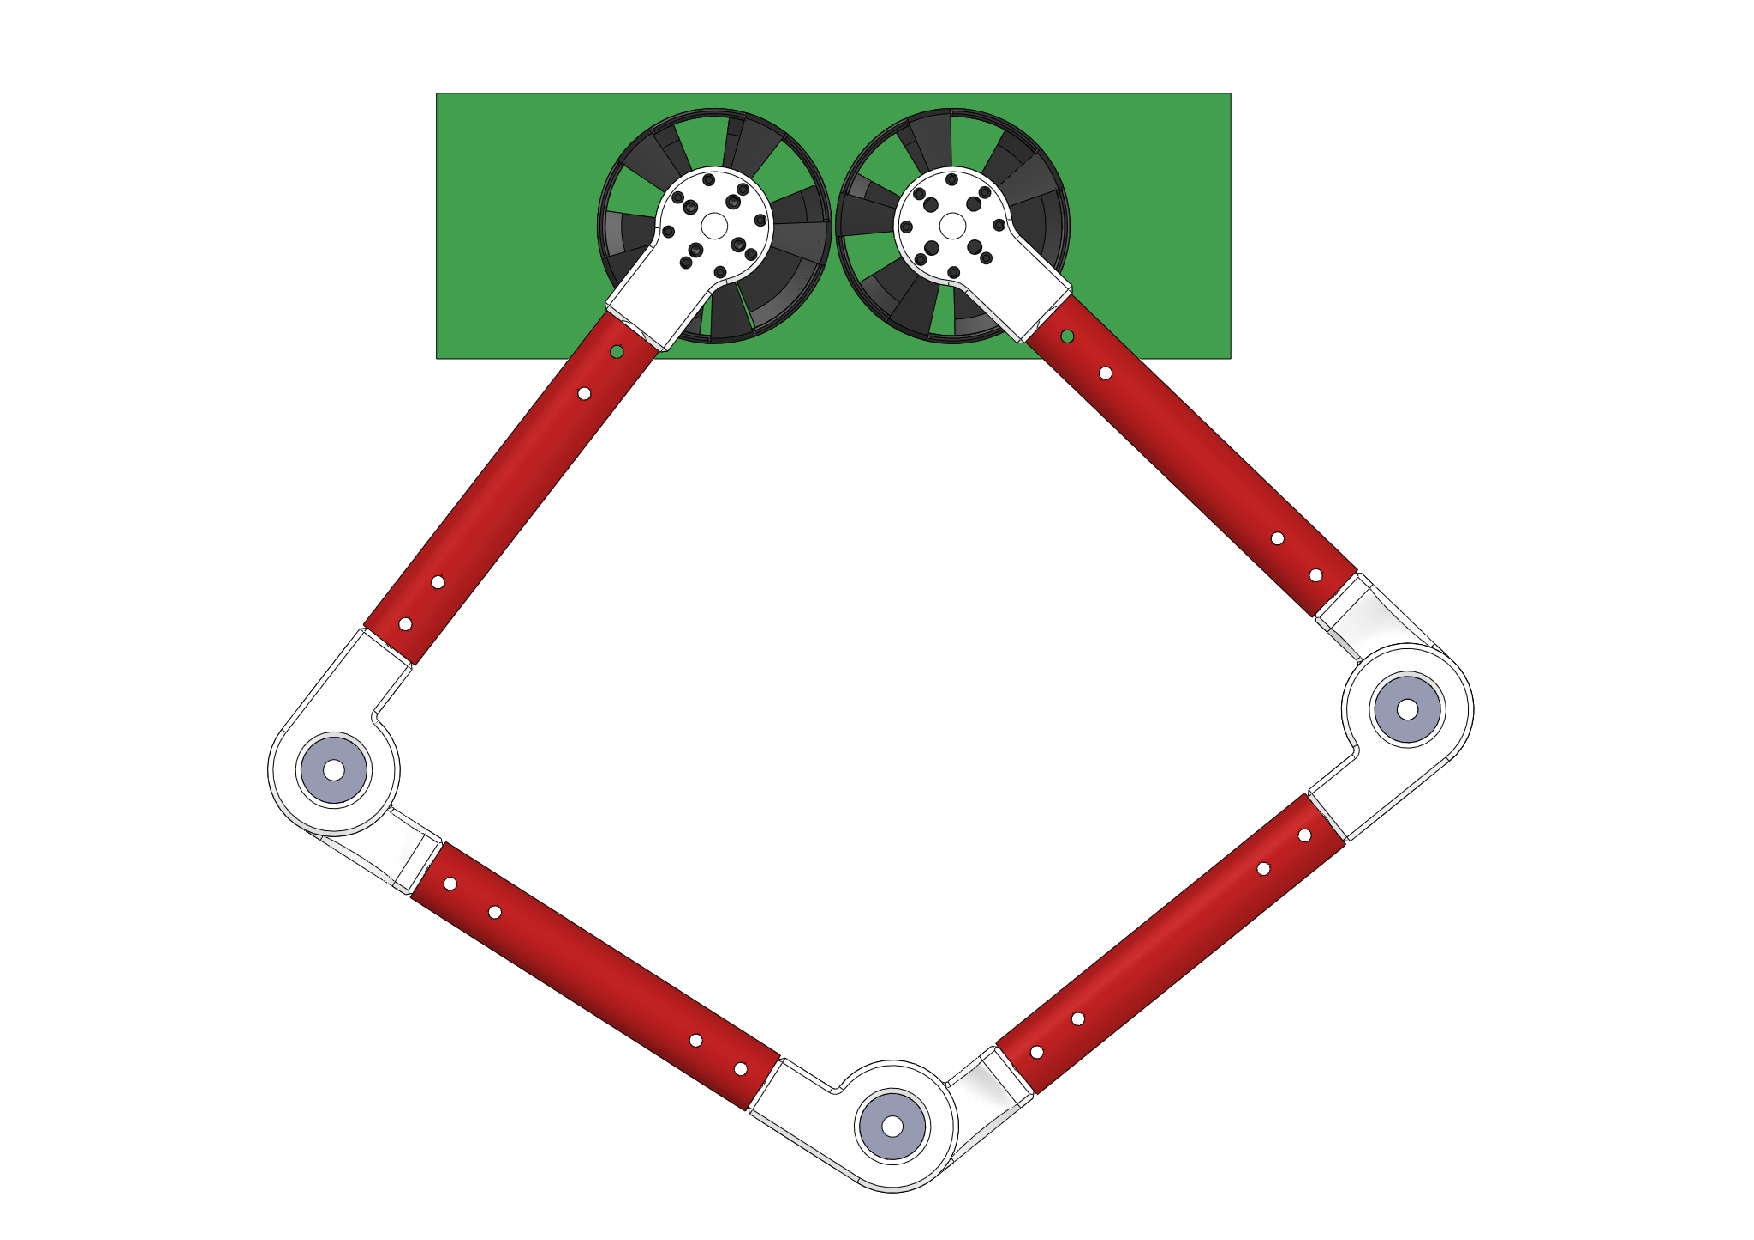
\includegraphics[width=0.5\textwidth,trim={0cm 0cm 0cm 0cm},clip]{images/mechanical/legsV1.pdf}
\caption{Version 1 of Baleka leg platform (Ben Bingham, 2016).}
\label{fig:legV1}
\end{figure}

The Mechatronics Lab has recently developed a single leg direct drive robot,
Baleka, to investigate modelling and control of rapid accelerations.
This project will involve the design of a control system to perform stable
hopping with the robot. Various controller algorithms will be investigated and
compared (eg. PID, MPC, etc.). The project will also involve developing a test
rig for the robot.

\section*{Deliverables}

\begin{itemize}
\item Mathematical model of the hopping robot must be developed in
Simulink/Matlab
\item Hopping controller design
\item Mechanical design of the test rig
\item Experimental testing of the robot
\end{itemize}

\section*{Skills/Requirements}

\begin{itemize}
\item Mathematical Modelling 
\item Mechatronics Design
\item Control Systems
\item Embedded Systems
\item Strong Practical and Mathematical skills required
\end{itemize}

\section*{ELO3: Engineering Design}

\textit{Perform creative, procedural and non-procedural design and synthesis of components, systems, engineering works, products or processes.}

The student is expected to design:

\begin{itemize}
\item Robot feedback control system
\item Rig for testing of hopping motion
\end{itemize}

\section*{Area of Research}

\begin{itemize}
\item Bio-inspired robotics
\item Control systems
\end{itemize}

\section*{Extra Information}

\url{http://ieeexplore.ieee.org/xpls/abs_all.jsp?arnumber=5648972}
\url{http://kodlab.seas.upenn.edu/uploads/Avik/compositionTR_sc.pdf}


\textsf{\tableofcontents}
%\tableofcontents

\listoffigures
\listoftables
\renewcommand\listoflistingscaption{List of Source Codes}
\listoflistings

%\printnomenclature

\mainmatter
%ch01: Introduction
%ch02: Literature Review
%ch03: Project Plan and Methodology
%ch04: Theory Development
%ch05: System Modelling and Simulation
%ch06: Conclusions
%ch07: Recommendations and Future Work

%\autoref{chap:intro}

\setchapterpreamble[uc][.75\textwidth]{%
\dictum[Lewis Carroll, \textit{Alice in Wonderland}]{%
``Begin at the beginning,'' the King said, gravely, ``and go on till you
come to an end; then stop.''}\vskip1em}

\chapter{Introduction}
\label{chap:intro}

With a hop, skip, and a jump -- the journey begins!

\section{Background}
\section{Objectives of the Study}
\subsection{Problems to be Investigated}
\subsection{Research Questions}
\subsection{Purpose of the Study}
\section{Scope and Limitations}
\section{Plan of Development}
\chapter{Literature Review}
\section{Legged Locomotion in Nature}
\section{Raibert Control}
\cite{Raibert1977}
\cite{Raibert1984}
\cite{Raibert1989}

\subsection{Dynamic Stability vs Static Stability}
\subsection{Phases of Motion}
\subsection{Leg Stance Control}
\section{Force Control}

\chapter{Project Plan and Methodology}
\lipsum
\chapter{Theory Development}

\section{General Co-ordinates}


\chapter{System Modelling and Simulation}
\chapter{Kinematics}

The 5-bar linkage design of the leg was first designed constructed in the study \cite{Duperret}. The geometry of the leg is fairly complex and the derivation of the kinematic equations equally so. J.M. Duperret and D.E. Koditschek derived the kinematic equations \cref{eq:forward-kinematics, eq:reverse-kinematics} in the study \cite{Duperret}. 

In this study the assumption was made that the distance $d$, as seen in \cref{fig:Geometric view of leg}, is zero. This simplifies the derivation of forward and reverse kinematic equations of the leg design by making the leg a 4-bar linkage. These kinematic equations are more easily calculated on board a microcontroller\cite{Duperret}, leaving more processing power for other control tasks if needed. 

The ease of calculation makes the loss in accuracy acceptable - in practise the simplified kinematic equations worked well with an insignificant calculation time made possible by the STM32F4's on-board floating point unit.

\begin{equation} \label{eq:forward-kinematics}
f(\phi_1, \phi_2) = \left(\begin{array}{c} \sqrt{{\mathrm{l_2}}^2 - {\mathrm{l_1}}^2\, {\sin\!\left(\frac{\mathrm{\phi_1}}{2} + \frac{\mathrm{\phi_2}}{2}\right)}^2} - \mathrm{l_1}\, \cos\!\left(\frac{\mathrm{\phi_1}}{2} + \frac{\mathrm{\phi_2}}{2}\right)\\
\frac{\mathrm{\phi_1}}{2} - \frac{\mathrm{\phi_2}}{2} \end{array}\right)
\end{equation}

\begin{equation} \label{eq:reverse-kinematics}
g(r, \theta) = \left(\begin{array}{c} \pi - acos(\frac{r^2 + l_1^2 - l_2^2}{2rl_1}) + \theta \\
\pi - acos(\frac{r^2 + l_1^2 - l_2^2}{2rl_1}) - \theta  \end{array}\right)
\end{equation}

\section{The Jacobian}
The Jacobian is formed by taking partial derivatives of the forward kinematic equation \cref{eq:forward-kinematics} as shown in \cref{eq:jacobian}. 

It is used as a mapping from the joint angles $\phi_1$ and $\phi_1$ to the end effector generalized coordinates $r$ and $\theta$. The Jacobian can be applied in robotic kinematic control to determine joint velocities and forces to achieve a desired force or velocity at the end effector, in this case the leg foot.

Taking the Jacobian of the kinematic mapping $f(\phi_1, \phi_2)$ the foot force vector, F, can be transformed to the motor torque commands, $\tau$:
\begin{equation} \label{eq:jacobian}
J = \left[ \frac{\partial \textbf{f}}{\partial \textbf{X}} \right] 
\end{equation}
where \textbf{X} = [r $\theta$].

\subsection{Velocity Mapping}

Velocity mapping from motor rotational velocity to polar velocity.
\begin{equation}
v(\dot{r}, \dot{\theta}) = J w(\dot{\phi_1}, \dot{\phi_2})
\end{equation}


\chapter{Geometric Simulation}

\begin{figure}
\centering
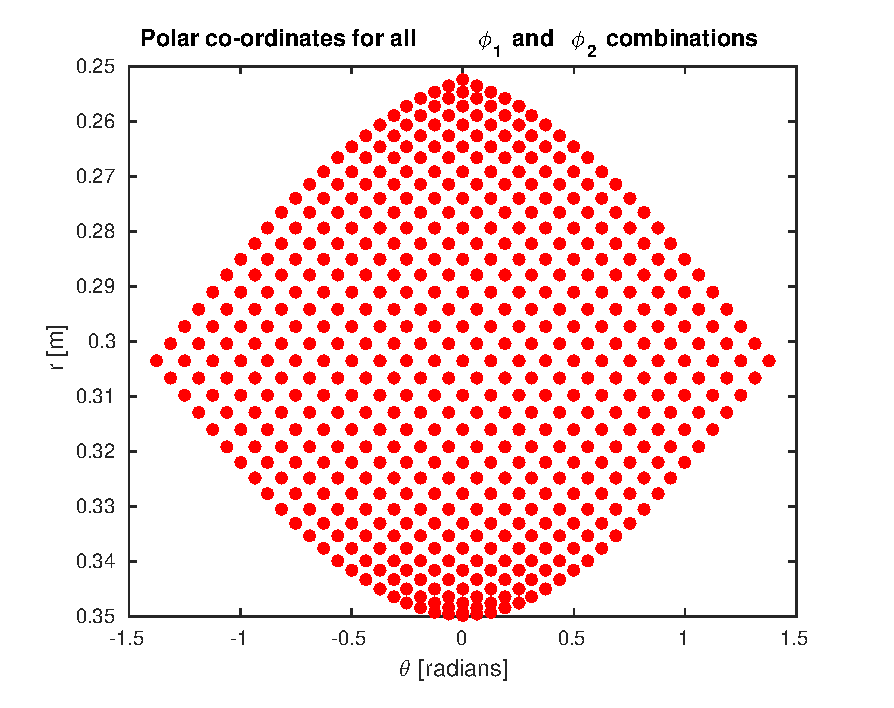
\includegraphics[width=1\textwidth]{images/geometry/forward-kinematic-leg-positions-5-30.eps}
\caption{Polar co-ordinates generated for all $\phi_1$ and $\phi_2$ combinations using forward kinematics: $l_1 = 5cm\ l_2 = 30cm$.}
\label{fig:Polar co-ordinates generated 5-30}
\end{figure}

\begin{figure}
\centering
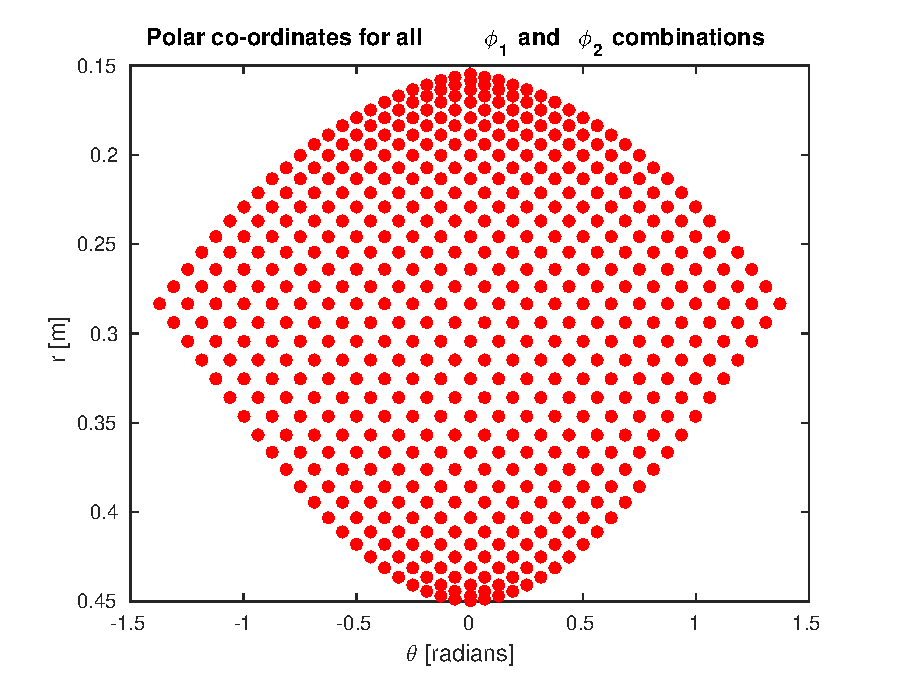
\includegraphics[width=1\textwidth]{images/geometry/forward-kinematic-leg-positions.eps}
\caption{Polar co-ordinates generated for all $\phi_1$ and $\phi_2$ combinations using forward kinematics: $l_1 = 15cm\ l_2 = 30cm$.}
\label{fig:Polar co-ordinates generated 15-30}
\end{figure}

\begin{figure}
\centering
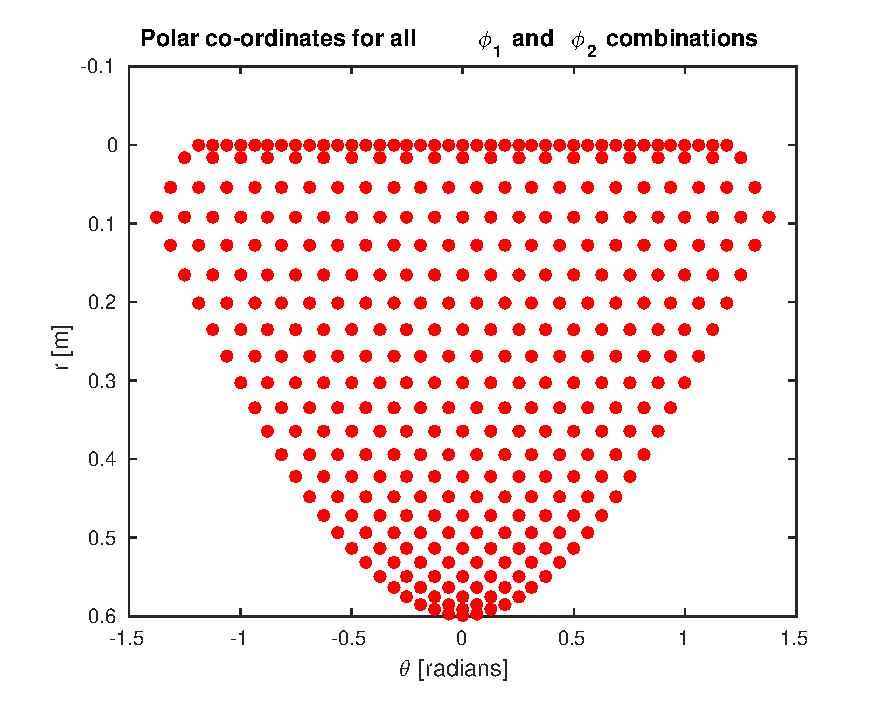
\includegraphics[width=1\textwidth]{images/geometry/forward-kinematic-leg-positions-30-30.eps}
\caption{Polar co-ordinates generated for all $\phi_1$ and $\phi_2$ combinations using forward kinematics: $l_1 = 30cm\ l_2 = 30cm$.}
\label{fig:Polar co-ordinates generated 30-30}
\end{figure}

\begin{figure}
\centering
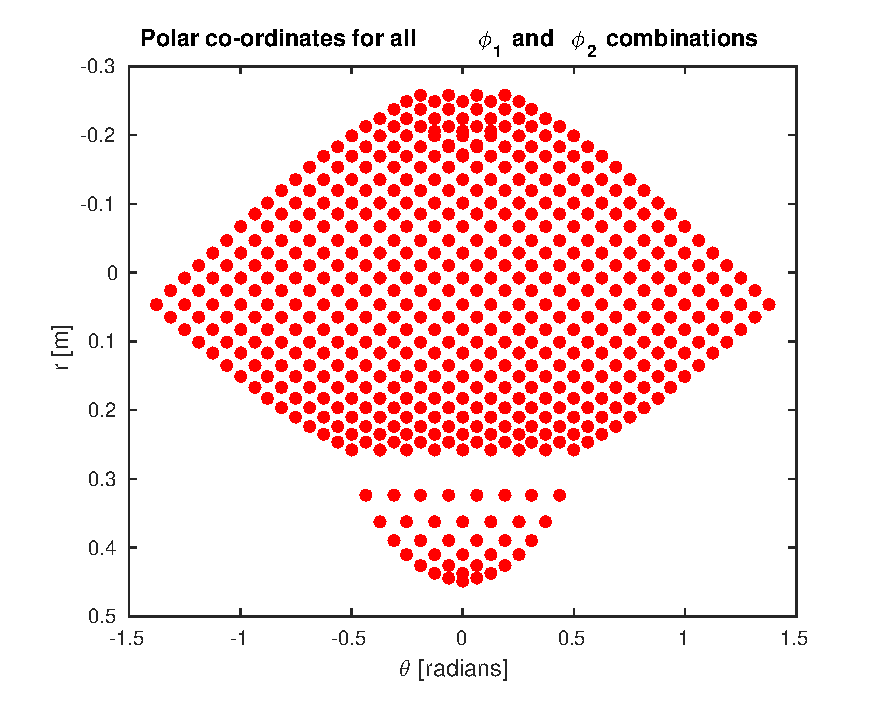
\includegraphics[width=1\textwidth]{images/geometry/forward-kinematic-leg-positions-30-15-complex.eps}
\caption{Polar co-ordinates generated for all $\phi_1$ and $\phi_2$ combinations using forward kinematics: $l_1 = 30cm\ l_2 = 15cm$.}
\label{fig:Polar co-ordinates generated 30-15}
\end{figure}
\chapter{Leg Design and Construction}

\begin{figure}[H]
\centering
\includegraphics[width=0.5\textwidth]{images/mechanical/leg-mount} 
\caption{Final leg design mounted to platform and linear guide.}
\label{fig:Final leg design}
\end{figure}

\section{Geometry}

\begin{figure}[H]
\centering
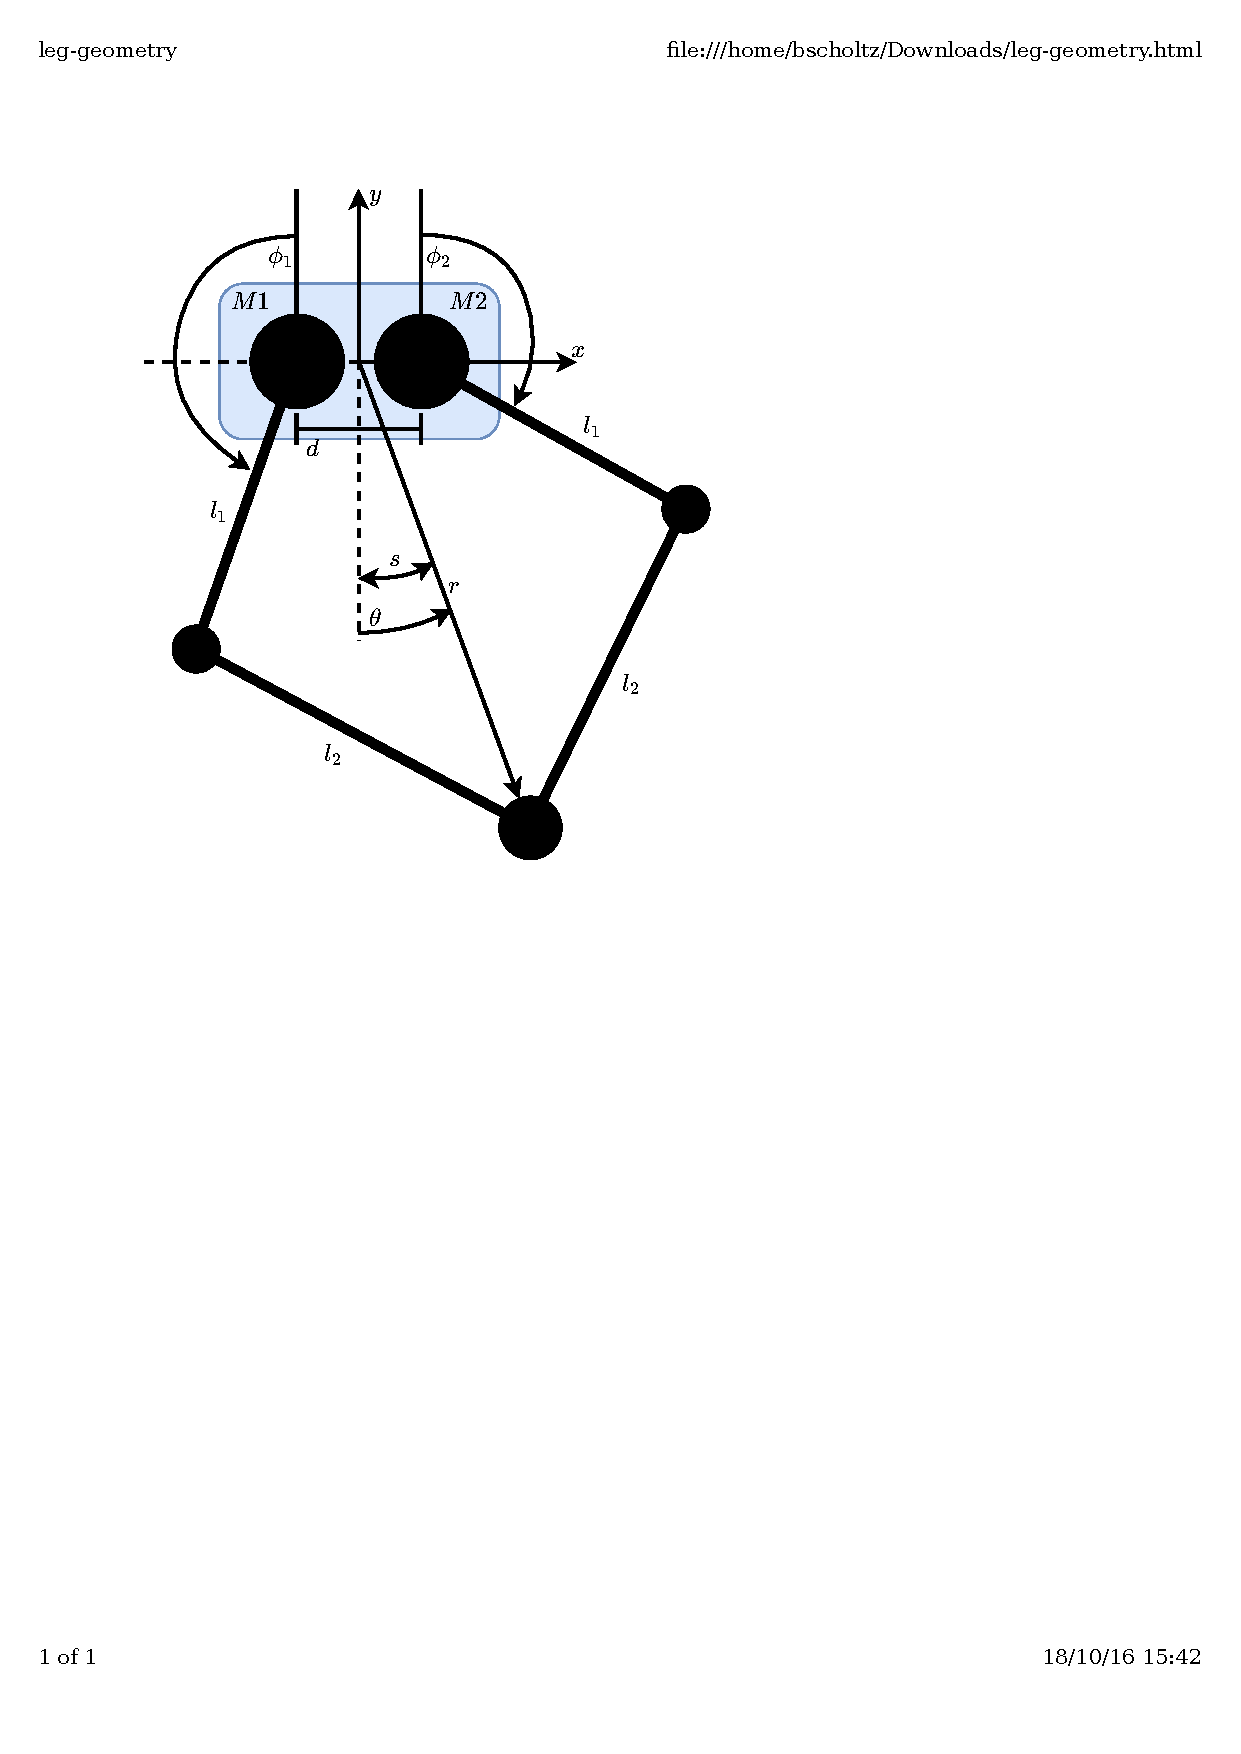
\includegraphics[clip, trim=2cm 15cm 7cm 2cm, page = 1, width=0.8\textwidth]{images/geometry/leg-geometry} 
\caption{Geometric view of leg.}
\label{fig:Geometric view of leg}
\end{figure}

\section{Mechanics and Construction}

\subsection{Alumnium Mounting Plate Design}

\begin{figure}
\centering
\subfloat[][CAD mounting plate V1.]{
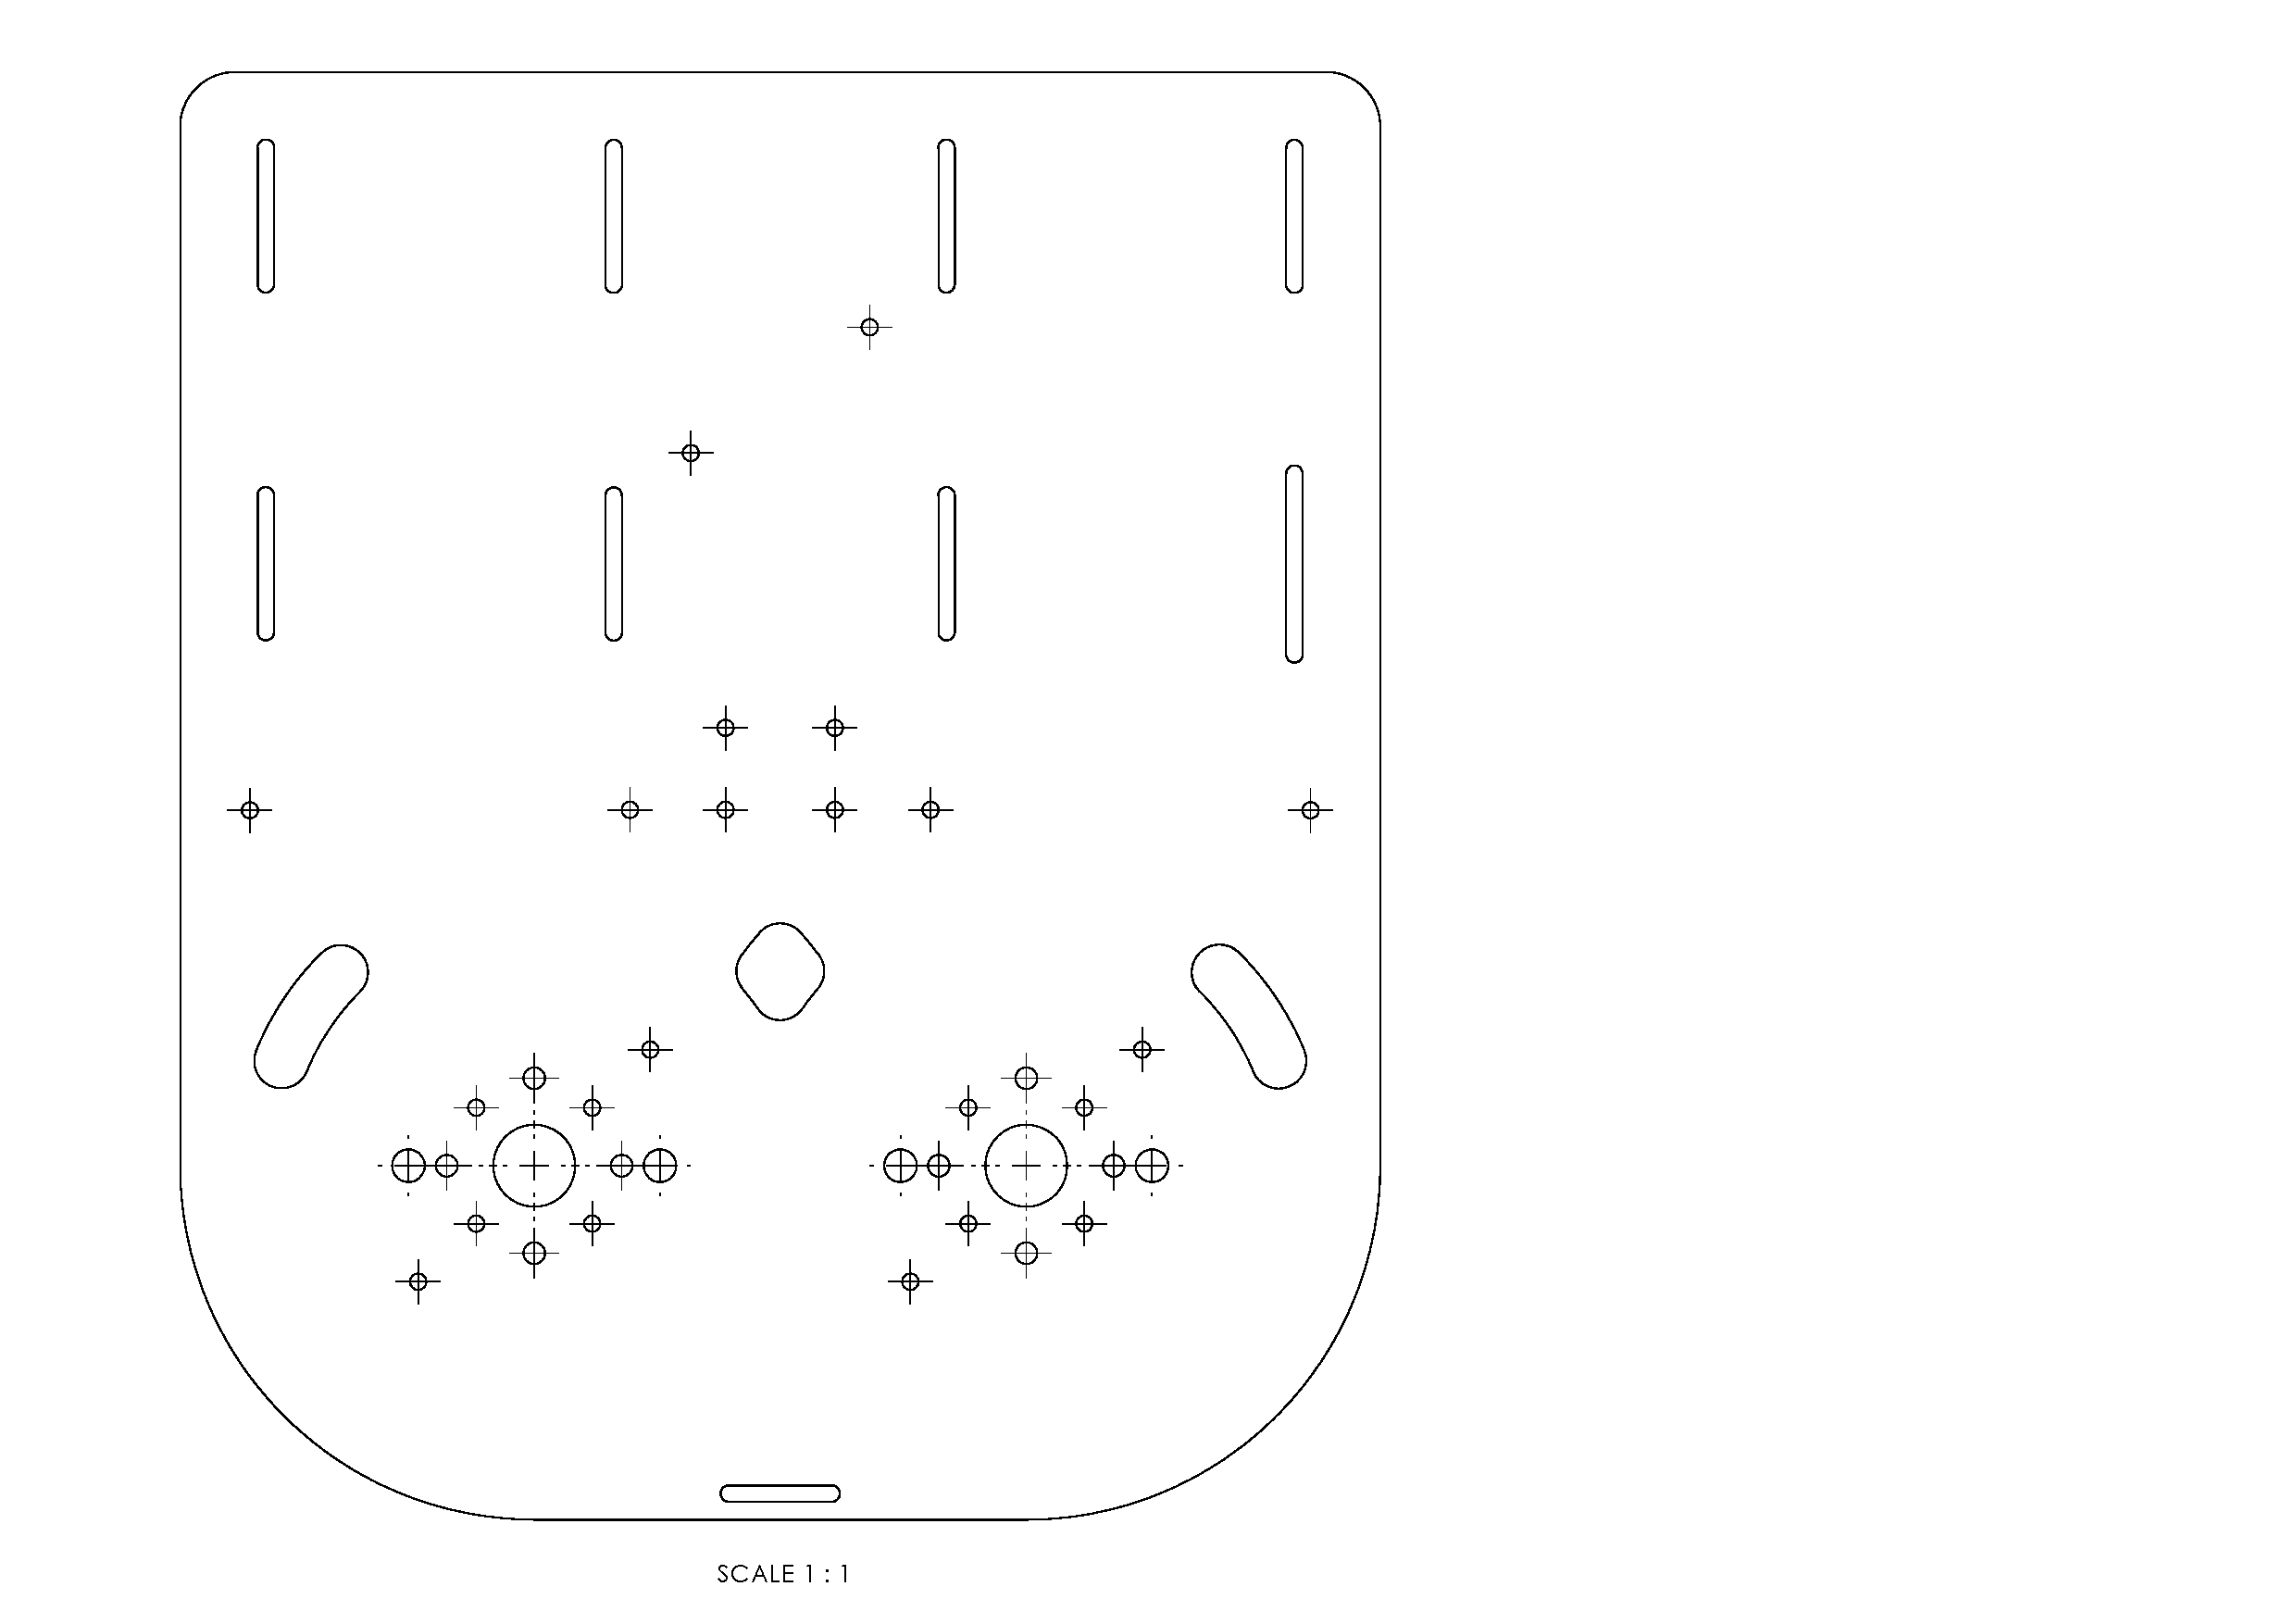
\includegraphics[clip, trim=2cm 0cm 16cm 1cm, page = 1, width=0.3\textwidth]{images/mechanical/laser-test-print-V1} 
\label{fig:CAD mounting plate V1}
}
\subfloat[][CAD mounting plate V3.1.3.]{
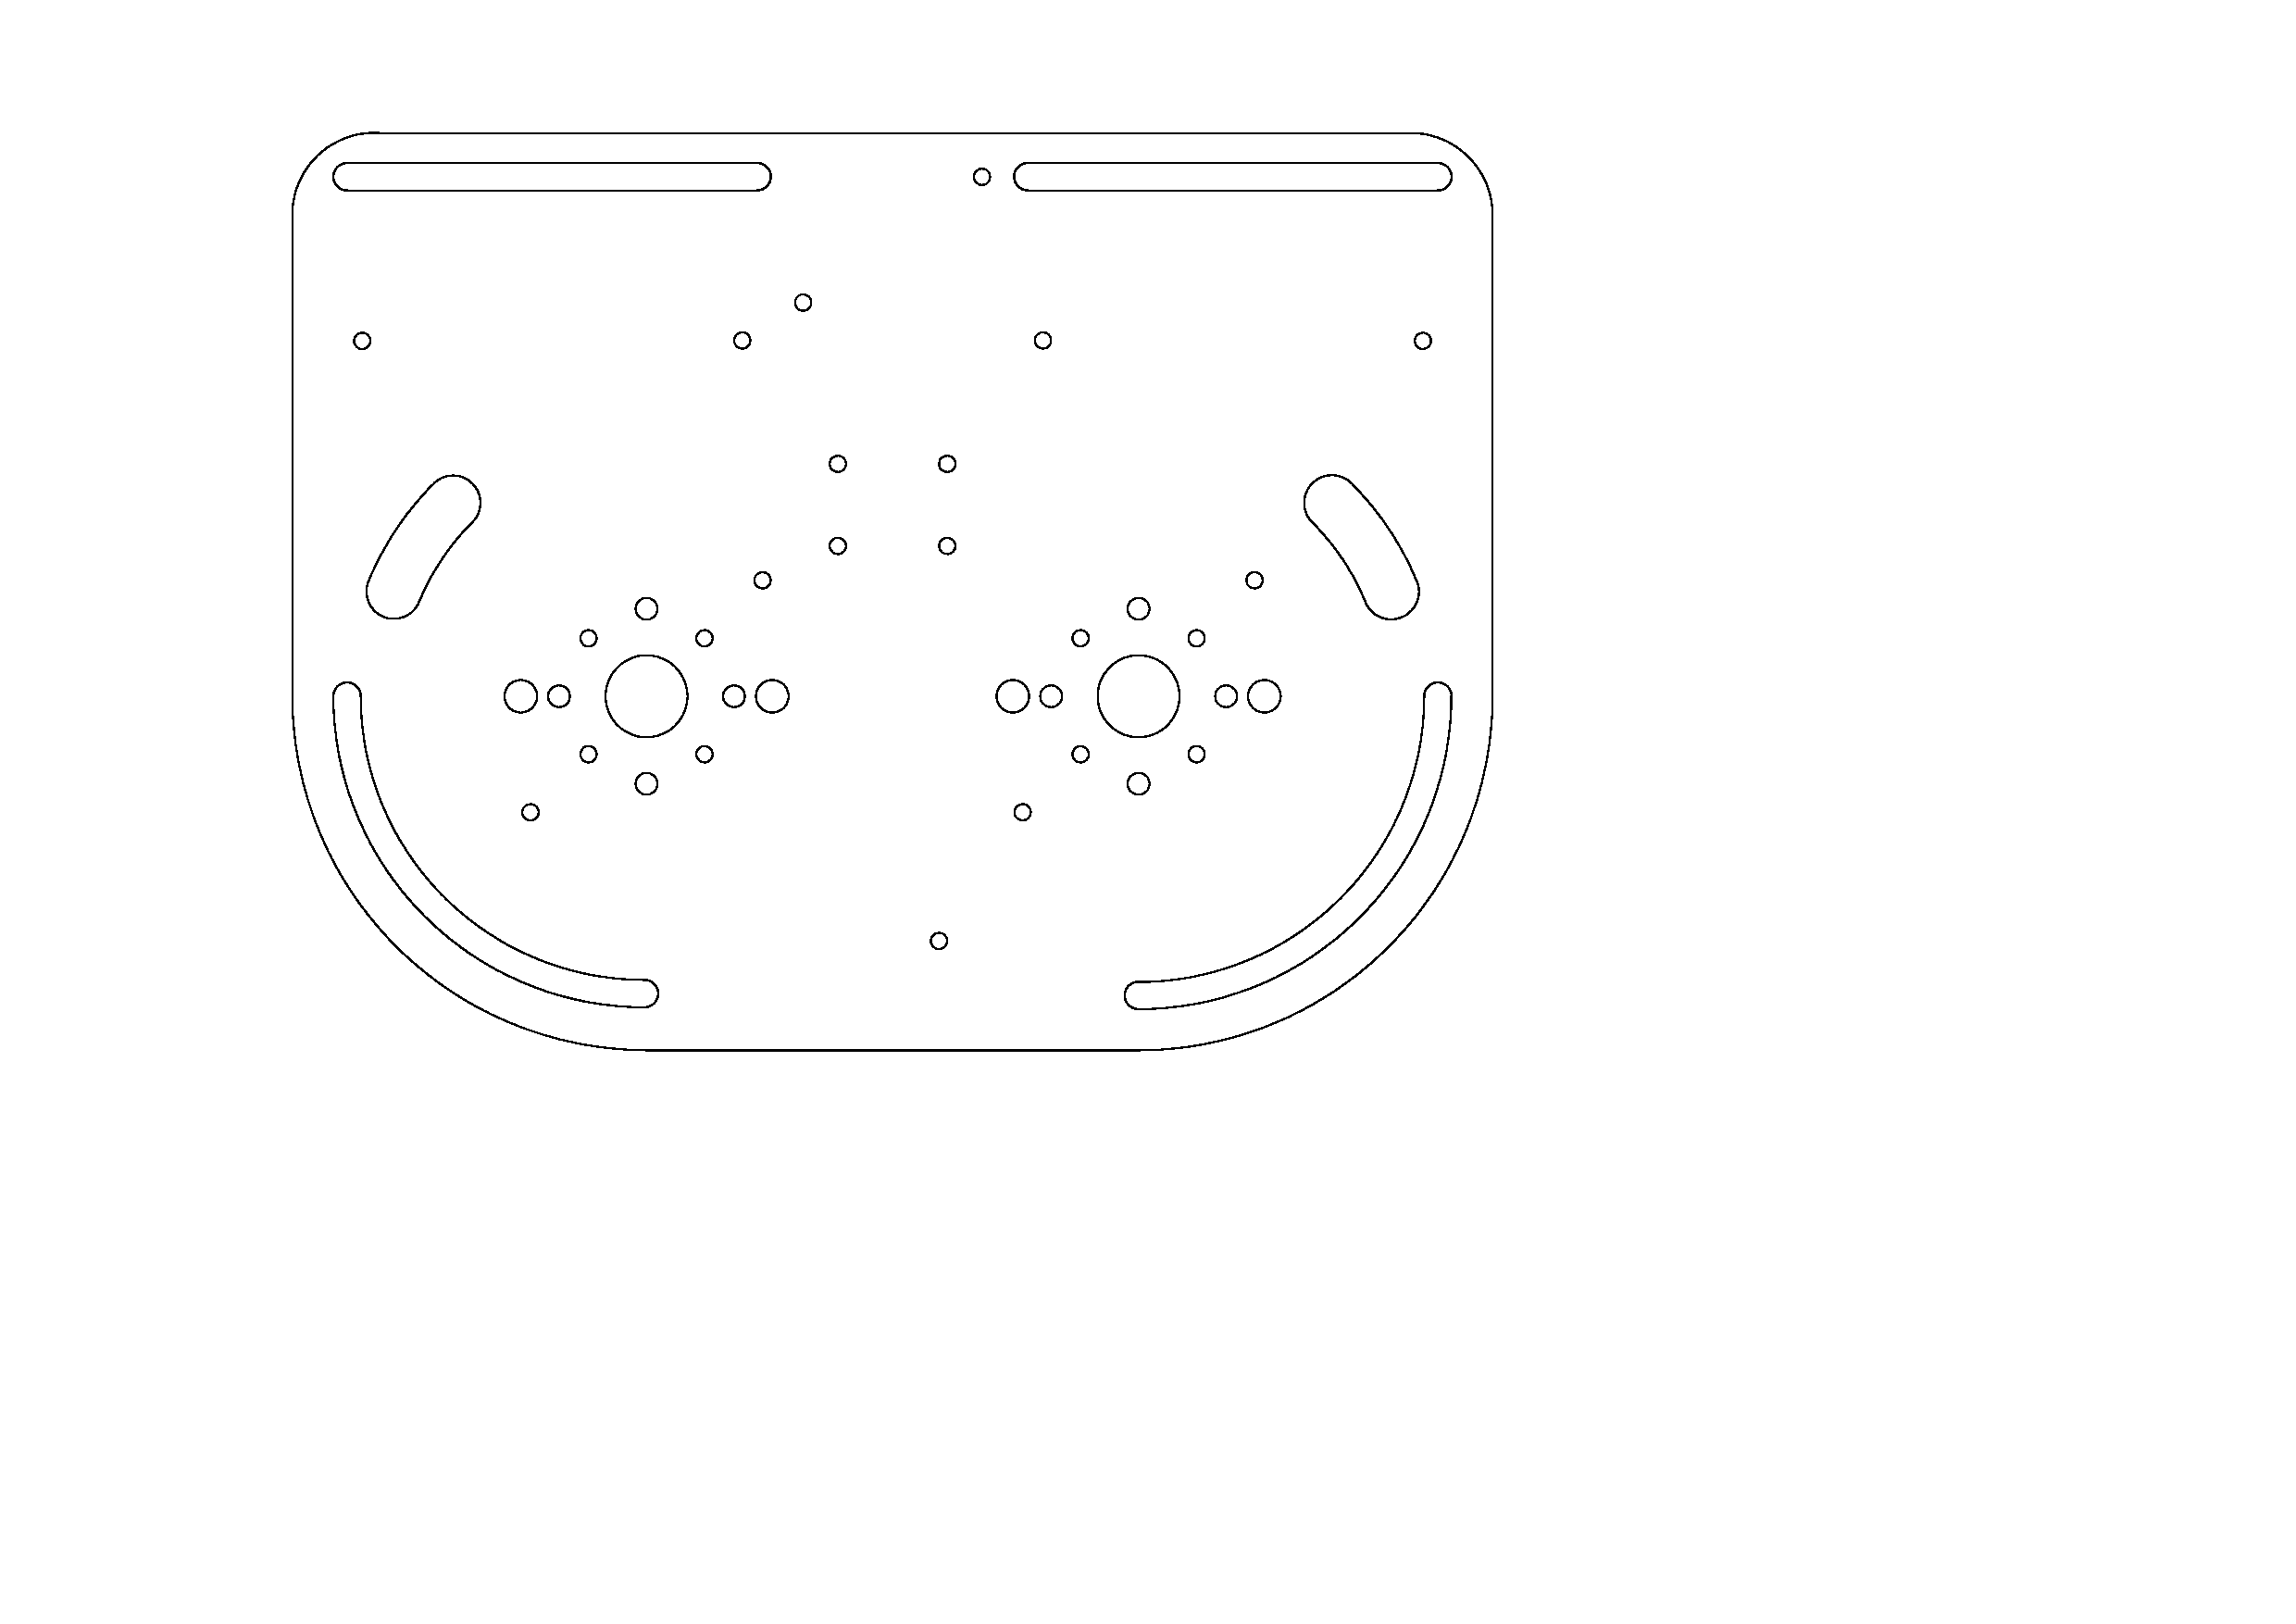
\includegraphics[clip, trim=5cm 10cm 14cm 2cm, page = 1, width=0.3\textwidth]{images/mechanical/laser-test-print-V313} 
\label{fig:CAD mounting plate V3.1.3}
}

\subfloat[][CAD mounting plate final design.]{
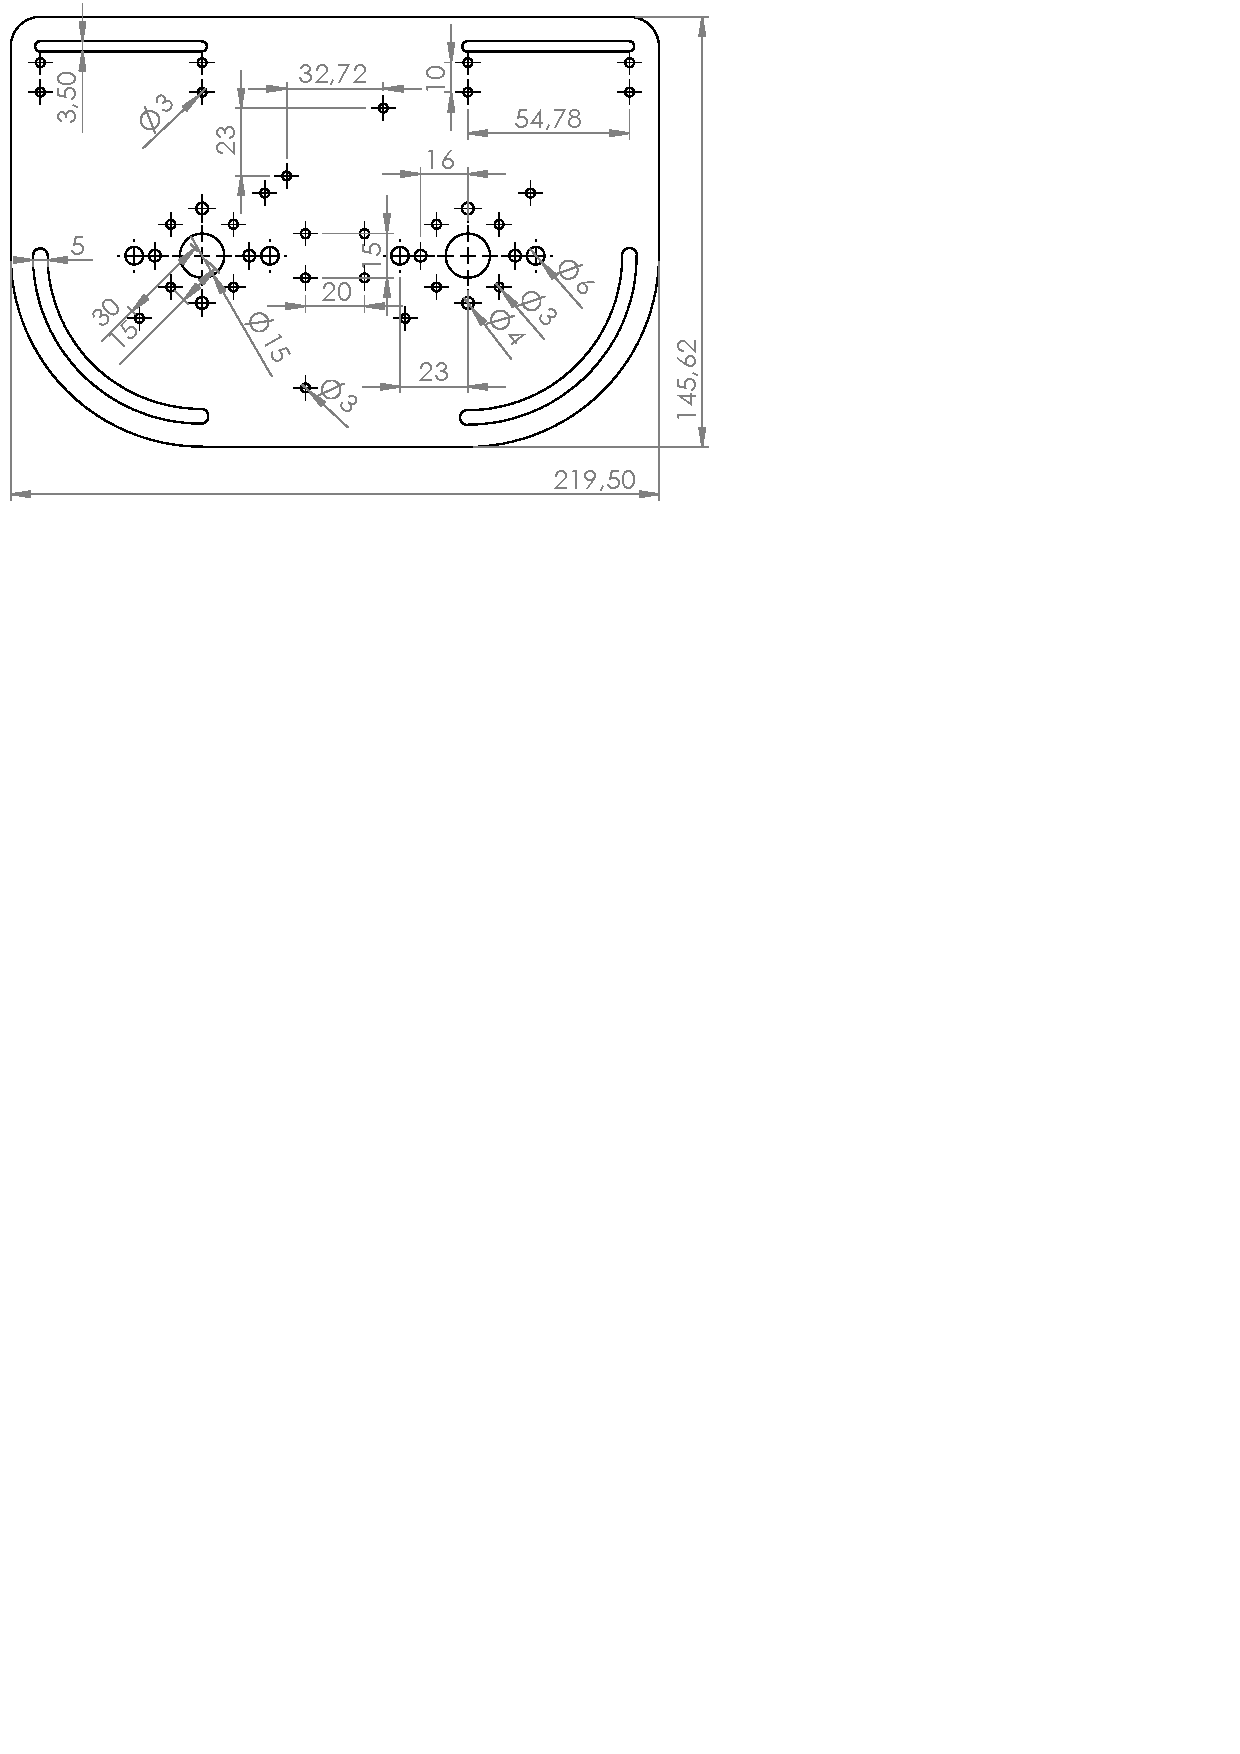
\includegraphics[clip, trim=0cm 21cm 9cm 0cm, page = 1, width=0.6\textwidth]{images/mechanical/main-plate-final} 
\label{fig:CAD mounting plate final design.}
}
\caption{Leg mounting plate iterations.}
\label{fig:Leg mounting plate iterations.}
\end{figure}

\begin{figure}
\centering
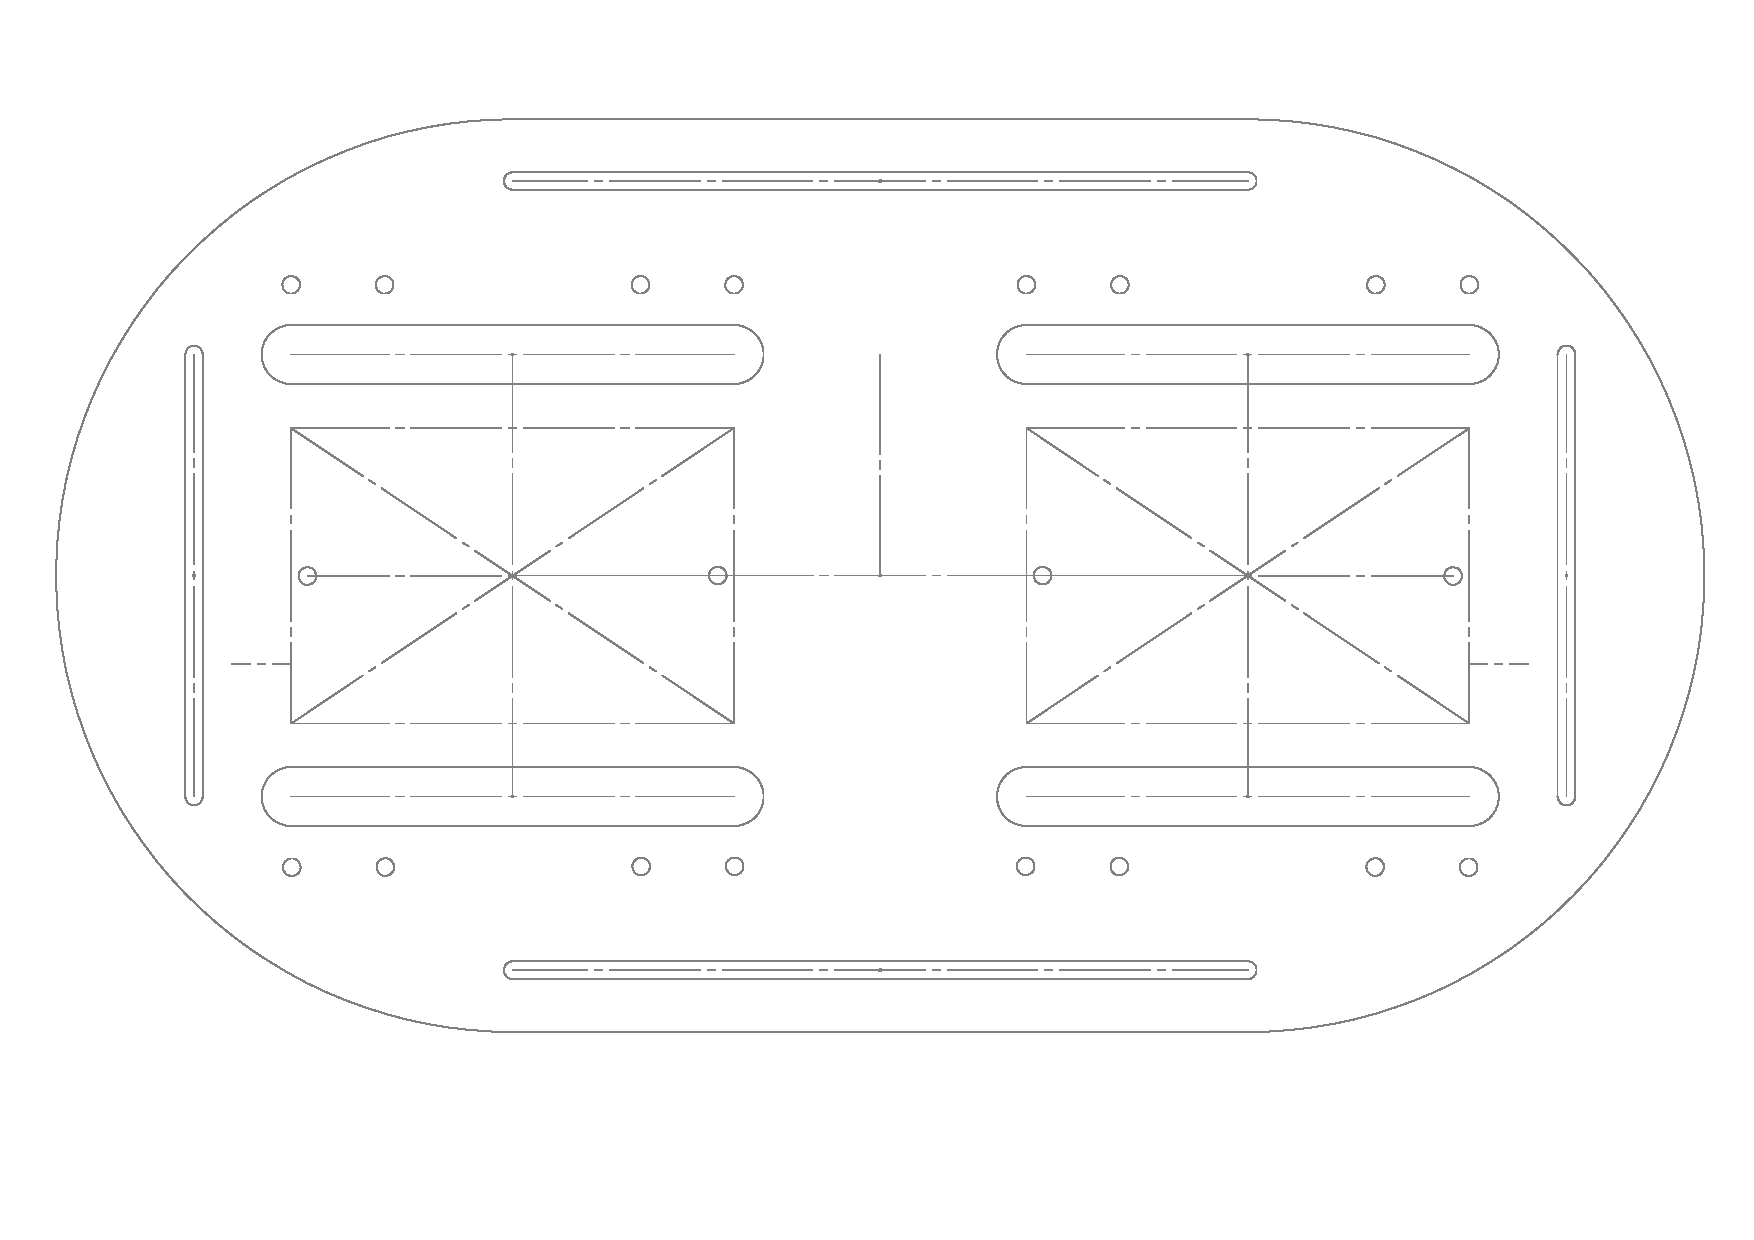
\includegraphics[width=0.6\textwidth]{images/mechanical/driver-mount-plate.pdf} 
\caption{Motor driver interface mounting plate.}
\label{fig:Motor driver interface mounting plate}
\end{figure}

\subsection{Linear Guide}
\begin{figure}
\centering
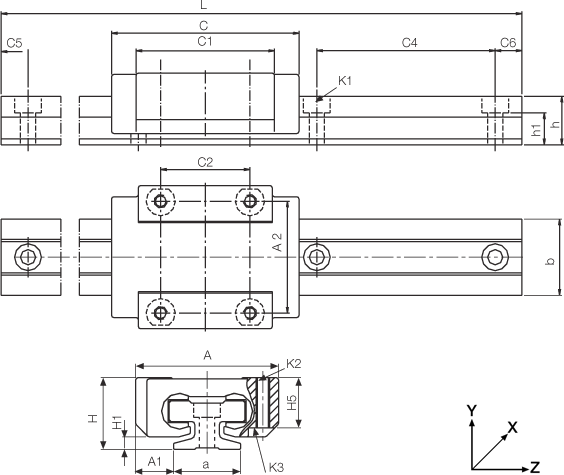
\includegraphics[width=0.8\textwidth]{images/mechanical/drylin-linear-guide.png} 
\caption{igus DryLin T - Low-profile linear guide.}
\label{fig:drylin-linear-guide}
\end{figure}

\subsection{CAD Robotic Leg Assembly}
\begin{figure}
\centering
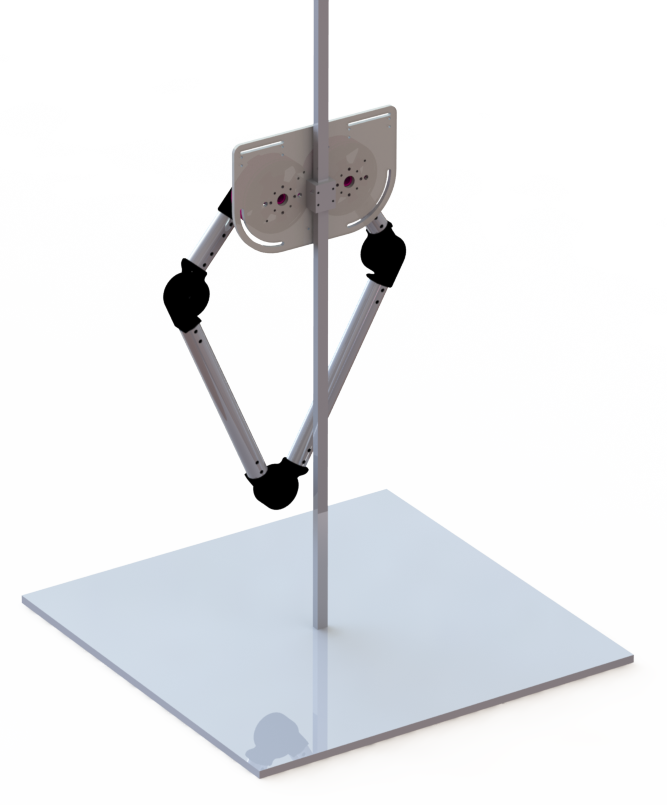
\includegraphics[width=0.8\textwidth]{images/mechanical/back-shot.png} 
\caption{Linear guide mounted leg model (CAD Solidworks assembly).}
\label{fig:Linear guide mounted leg model}
\end{figure}

\section{Electronics and Communication}
\subsection{Accelerometer and Gyroscope}
\subsection{Distance Sensor}
\subsection{Microcontroller}
\section{Communication Interfaces}
\subsection{Shielding}
\section{Motors and Drivers}

\subsection{Driver Selection}

\begin{figure}
\centering
\subfloat[][AMC DigiFlex Performance Servo Drive.]{
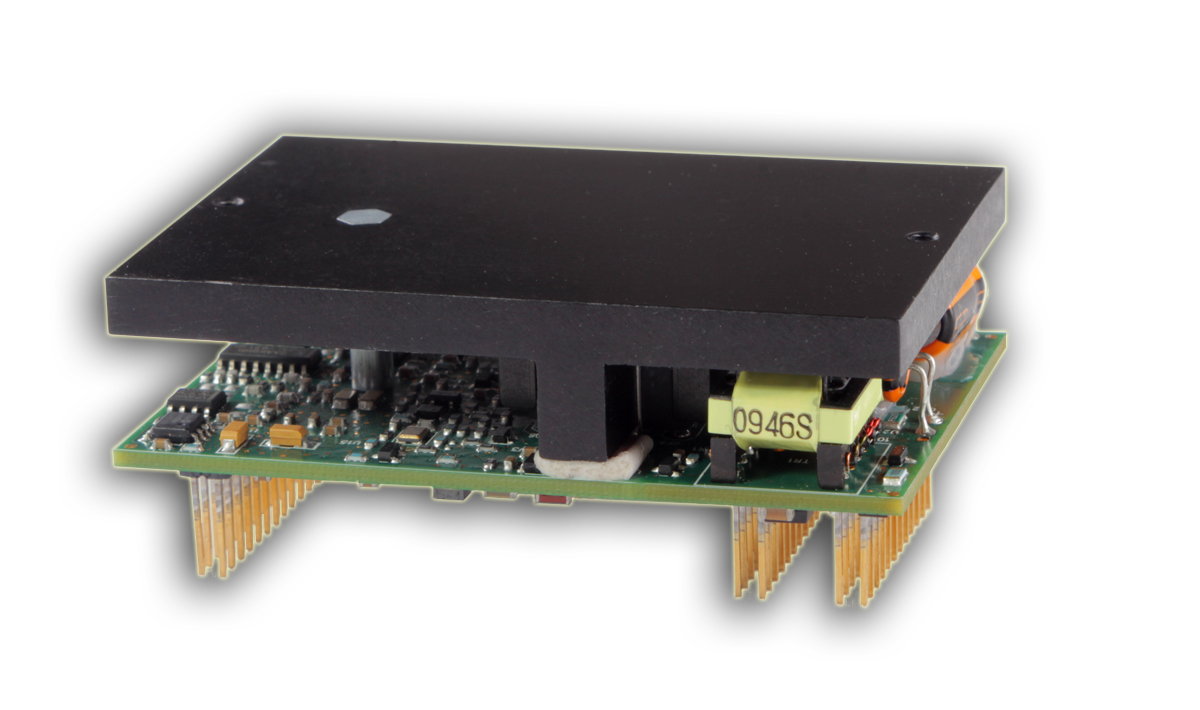
\includegraphics[width=0.5\textwidth]{images/driver/driver.jpg} 
}
\subfloat[][AMC DigiFlex Performance Servo Drive mounting card.]{
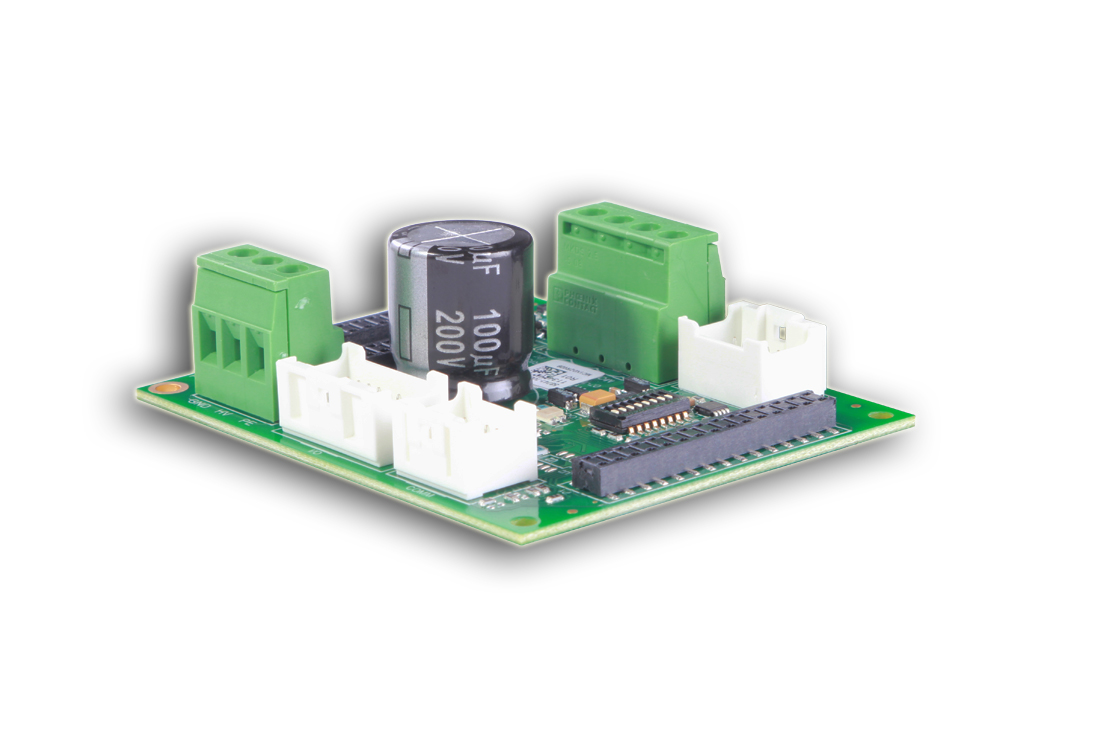
\includegraphics[width=0.5\textwidth]{images/driver/mounting-card.jpg}
} 
\caption{AMC Servo Drive and Mounting Card.}
\label{fig:AMC Servo Drive and Mounting Card}
\end{figure}

\subsection{Motor Selection}

\begin{figure}
\centering
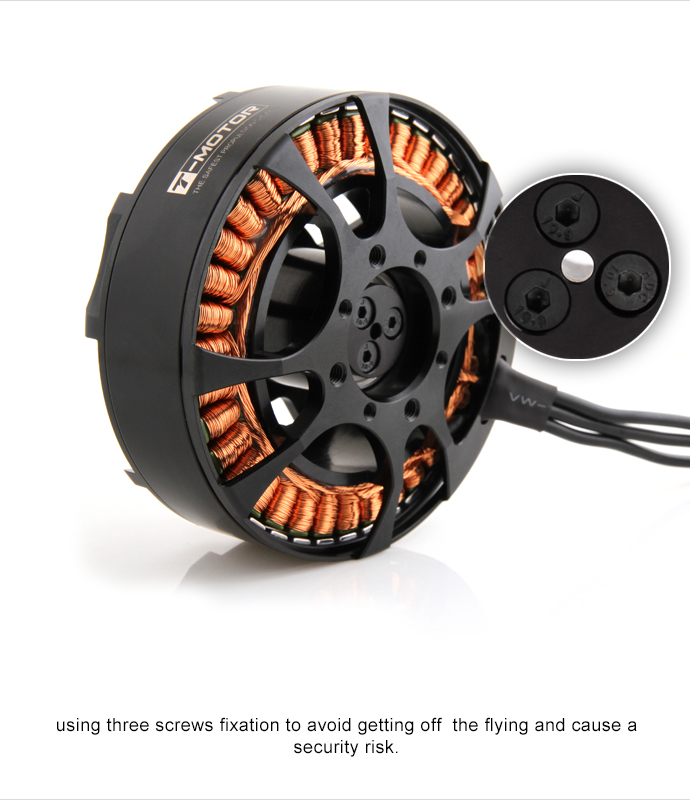
\includegraphics[clip, trim=0cm 5cm 0cm 2cm, width=0.4\textwidth]{images/motor/TMotorU10Plus} 
\caption{T-Motor U10 Plus Brushless DC Motor.}
\label{fig:TMotorU10Plus}
\end{figure}

\subsection{Motor Model Calculations}

\subsubsection{Experimental Calculation of $K_t$ and $K_e$}
The motor torque constant, $K_t$, was calculated using the torque current relation $\tau = K_tI$. The leg was modelled as a virtual spring-damper system, as seen in \cref{fig:Leg spring-damper virtual model}. 

The spring constant, $K_{s1}$, was set to $200\ [N/m]$, and the damping and torsional spring-damping constants were set to zero. $K_t$ was tuned until the theoretical foot force matched the practical foot force measured via a scale. The leg was fixed at a set height imposing a radial offset on the virtual spring-damper system.

For a spring constant of $200\ [N/m]$ and a radial offset of $0.15\ m$ a theoretical foot force of $K_{s1}\Delta r = 30\ N$ was expected. A mass of approximately $3\ kg$ was measured with $K_t = 0.08\ [Nm/A]$ set in the virtual leg model controller, resulting in a foot force of $3\ kg \times 9.81\ m/s^2 = 29.43\ [N]$. 

The study in \cite{Kalouche2016}, using the same T-Motor U10 Plus motors, calculated a torque constant of $K_t =  0.072\ [Nm/A]$. This confirms the experimental results obtained above.

For an ideal motor at a constant operating point, $K_e$ will equal $K_t$, as shown in \cref{eqn:ktke}.

\begin{equation} \label{eqn:ktke}
\begin{aligned}
&V_t = K_e\omega_m + IR_m \\
&\tau_m = K_t I \\
&P_{elec.} = V_t I = K_e \omega_m I + I^2 R \\ 
&P_{mech.} = \tau_m \omega_m = K_t I \omega_m \\
&P_{loss.} = I^2 R_m \\
&P_{elec.} = P_{mech.} + P_{loss.} \\
&\therefore K_e\ [V/rad/s]= K_t\ [Nm/A] = 0.08
\end{aligned} 
\end{equation}

\subsubsection{Calculation of $R_m$ and $L_m$}
The resistance and inductance of the 3 phase windings of the motor were calculated using a lab multimeter to be $R_m = 47.5\ m\Omega$ and $L_m = 35\ \mu H$ respectively. 

Brushless DC motor windings are usually connected in WYE formation, as seen in \cref{bldc-wye-connection}. This means the measured values for resistance and inductance were line-to-line values and had to be divided by two to get the per phase values above.

\begin{figure}
\centering
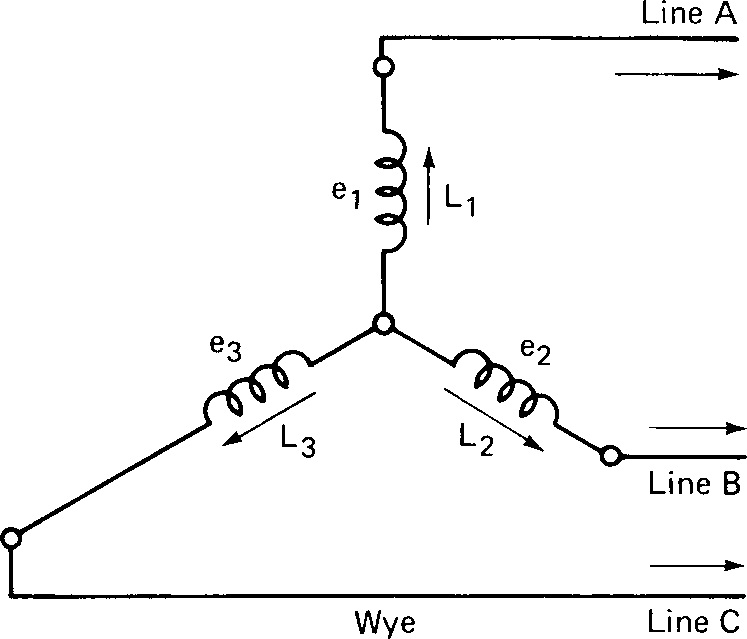
\includegraphics[width=0.4\textwidth]{images/motor/wye.jpg} 
\caption{WYE connected BLDC motor windings.}
\label{fig:bldc-wye-connection}
\end{figure}

\subsubsection{Calculation of $J_m$}
In order to calculate the moment of inertia of the motor, $J_m$, the ratio of acceleration torque to acceleration to steady state needs to be found. By commanding a DC equivalent current input of $1\ A$ and measuring the time taken to reach a steady state velocity, \cref{eqn:Jm} can be used to calculate $J_m$. The velocity vs. time plot used can be seen in \cref{fig:jm-plots}.

\begin{equation} \label{eqn:Jm}
\begin{aligned}
J_m &= \frac{T_{acc.}[N/m]}{a[m/s^2]} \\
&= \frac{IK_t}{a} \\
&= \frac{IK_t}{\frac{\Delta v}{\Delta t}}\ [kg/m^2]
\end{aligned}
\end{equation}

where $I=1\ A$, $K_t=0.08\ Nm/A$, $\Delta v = 1313.906\times \frac{2\pi}{60}\ rad/s$ and $\Delta t = 588.889\times10^{-3}\ s$.

This results in a motor moment of inertia of $J_m = 3.424 \times 10^{-4}\ [kg/m^2]$.

\subsubsection{Calculation of $B_m$}

The motor damping or viscous friction, $B_m$, was assumed to be negligible. Brushless DC motors have near zero damping and will have little effect on the simulated motor model.

\begin{figure}
\centering
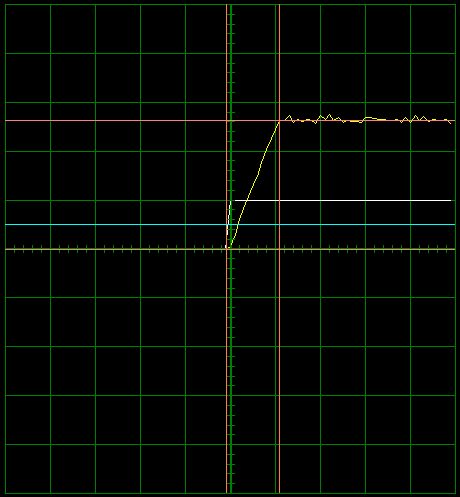
\includegraphics[width=0.5\textwidth]{images/driveware/current-velocity-response} 
\caption{Velocity vs. time plot for 1A equivalent DC command.\\
(500 rpm; 500 ms/div)}
\label{fig:jm-plots}
\end{figure}

\subsubsection{Calculation of $\tau_e$ and $\tau_m$}
The electrical and mechanical time constants of the motor, $\tau_e$ and $\tau_m$ respectively, can be used to plot a root-locus plot with poles at $-\tau_e$ and $-\tau_m$ as can be seen in \cref{...}. This is useful when designing a current controller for the system. $\tau_e$ and $\tau_m$ can be calculated using \cref{eqn:motor-time-constants}.

\begin{equation} \label{eqn:motor-time-constants}
\begin{aligned}
&K_m = \frac{1}{B_m} \\
&\tau_m = \frac{J_m}{B_m} \\
&K_e = \frac{1}{R_m} \\
&\tau_e = \frac{L_m}{R_m} 
\end{aligned}
\end{equation}

From \cref{eqn:motor-time-constants} and using the previously calculated motor constants, $\tau_e = 7.368 \times 10^{-4}$ and $\tau_m = 3.424 \times 10^{-4}$. This is assuming a motor viscous friction of $B_m = 0$.

The resulting motor model open loop root-locus plot can be seen in \cref{fig:ol-motor-rlocus}. As expected the system has only negative real roots and will be stable in open loop.

\begin{figure}
\centering
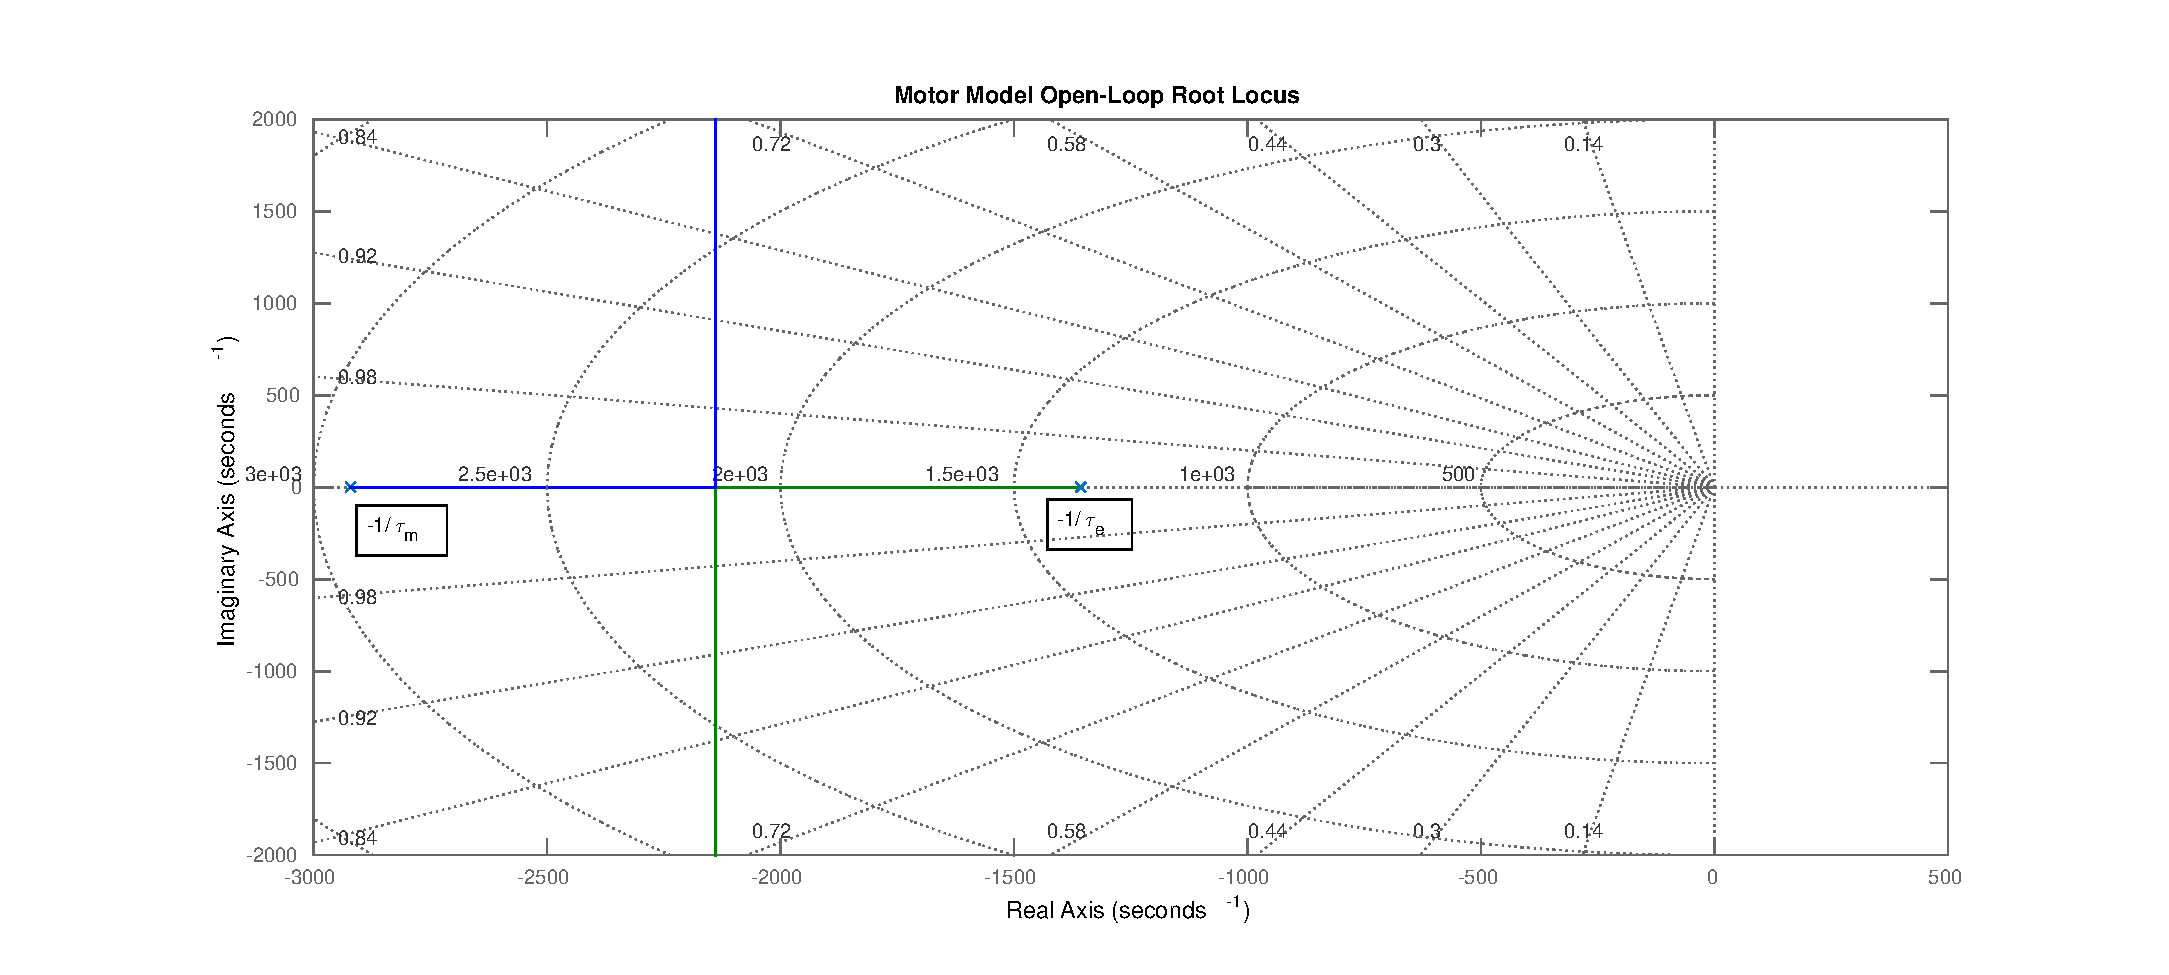
\includegraphics[width=1\textwidth]{images/motor/ol-motor-rlocus} 
\caption{Motor model open loop root-locus plot.}
\label{fig:ol-motor-rlocus}
\end{figure}


\subsection{Driver Configuration}

The AMC drivers allow extensive customisation. After the motor, encoder, and general communication control parameters are configured, the PID control loops of the drivers can be configured, as seen in \cref{fig:AMCControlLoops}.

The motor drivers were initially configured with both on-board PID current and position control loops enabled. This allowed initial modelling of the motors, configuring of the motor encoders, and determining of the position limits (in counts). For control of the leg, the position control loop was finally implemented on the STM32F4 microcontroller, while using the existing current control loop of the motor drivers.

The AMC drivers were configured using the AMC Driveware configuration software, which provided an oscilloscope to measure the relevant motor responses as seen in \cref{fig:jm-plots,,fig:current-tuning-plots,,fig:position-tuning-plots}.

\begin{figure}
\centering
\includegraphics[clip, trim=2cm 5cm 2cm 8cm, page = 114, width=1\textwidth]{pdfs/AMC_DriveWareSoftwareManual.pdf} 
\caption{AMC DigiFlex Performance Servo Drive control loops (AMC, 2014).}
\label{fig:AMCControlLoops}
\end{figure}

\subsubsection{Current Control Loop}

By using a 1 A 120Hz square wave current command the current PI control loop was tuned, as seen in \cref{fig:current-tuning-plots}. Initially both  the proportional gain, $K_p$, and the integral gain, $K_i$, were set to zero. $K_p$ was slowly increased until the final amplitude of the current output just started to overshoot. $K_i$ was then set to minimize the steady state error. 

Values of $K_p = 0.277$ and $K_i = 0.262$ were obtained. Both motors were found to operate optimally with the same PI gain values.

\begin{figure}
\centering
\subfloat[][Motor driver current loop pre-tuning.\\ 
(200 mA; 5 ms/div)]{
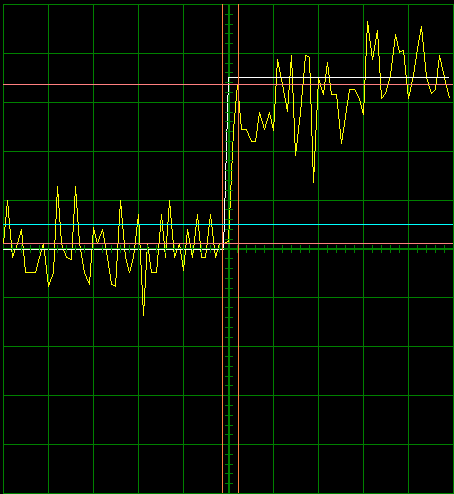
\includegraphics[width=0.5\textwidth]{images/driveware/current-pre-tuning-plot.png} 
}
\subfloat[][Motor driver current loop tuning - 1A 120Hz square wave command.\\(1 A; 1 ms/div)]{
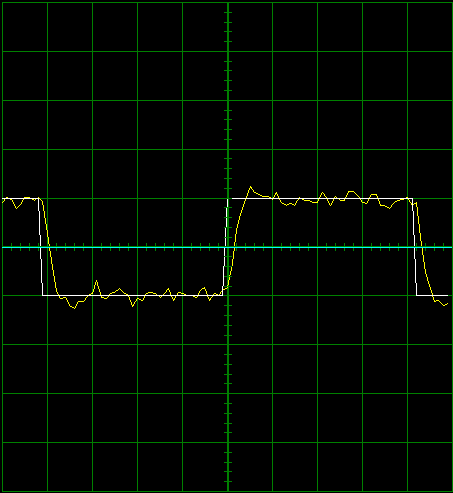
\includegraphics[width=0.5\textwidth]{images/driveware/current-tuning-plot.png} 
}
\caption{Motor driver current loop tuning plots.}
\label{fig:current-tuning-plots}
\end{figure}

\subsubsection{Position Control Loop}
The on-board AMC motor driver control loop was set up to test the encoder configuration. The encoder and relevant position limits can be seen in \cref{sec:motor-encoders}. 

A 1Hz sinusoid was used to tune the PID control loop gains. Values of $K_p = 0.0005793$, $K_i = 0.0006052$ and $K_d = 2.769e-9$ were found to achieve optimal set-point tracking as seen in \cref{fig:position-tuning-plots}. The sinusoidal set-point can be seen in white and the position feedback in yellow. A 10-30 ms lag time can be seen due to the inertial load. This lag time causes a dead-band which should be considered when implementing a controller. 

These tests were performed with the leg attached - the inertial load provided by the leg made PID control loop tuning possible, whereas without any inertial load the BLDC motors overshot their set-point.

\begin{figure}
\centering
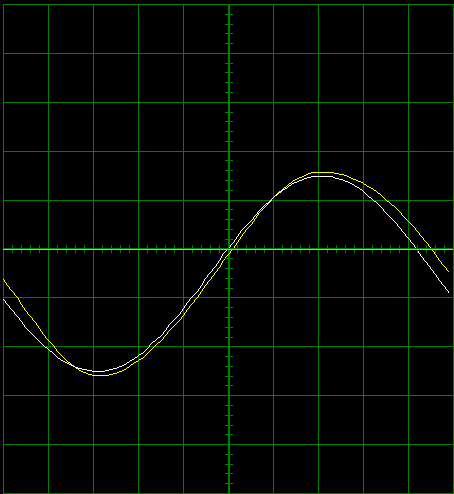
\includegraphics[width=0.5\textwidth]{images/driveware/position-tuning-plot} 
\caption{Motor driver position loop tuning - (-350:200) count 1Hz sinusoid command with 300 count offset.\\(100 ct; 100 ms/div)}
\label{fig:position-tuning-plots}
\end{figure}

\subsection{Motor Encoders}
\label{sec:motor-encoders}

\begin{figure}
\centering
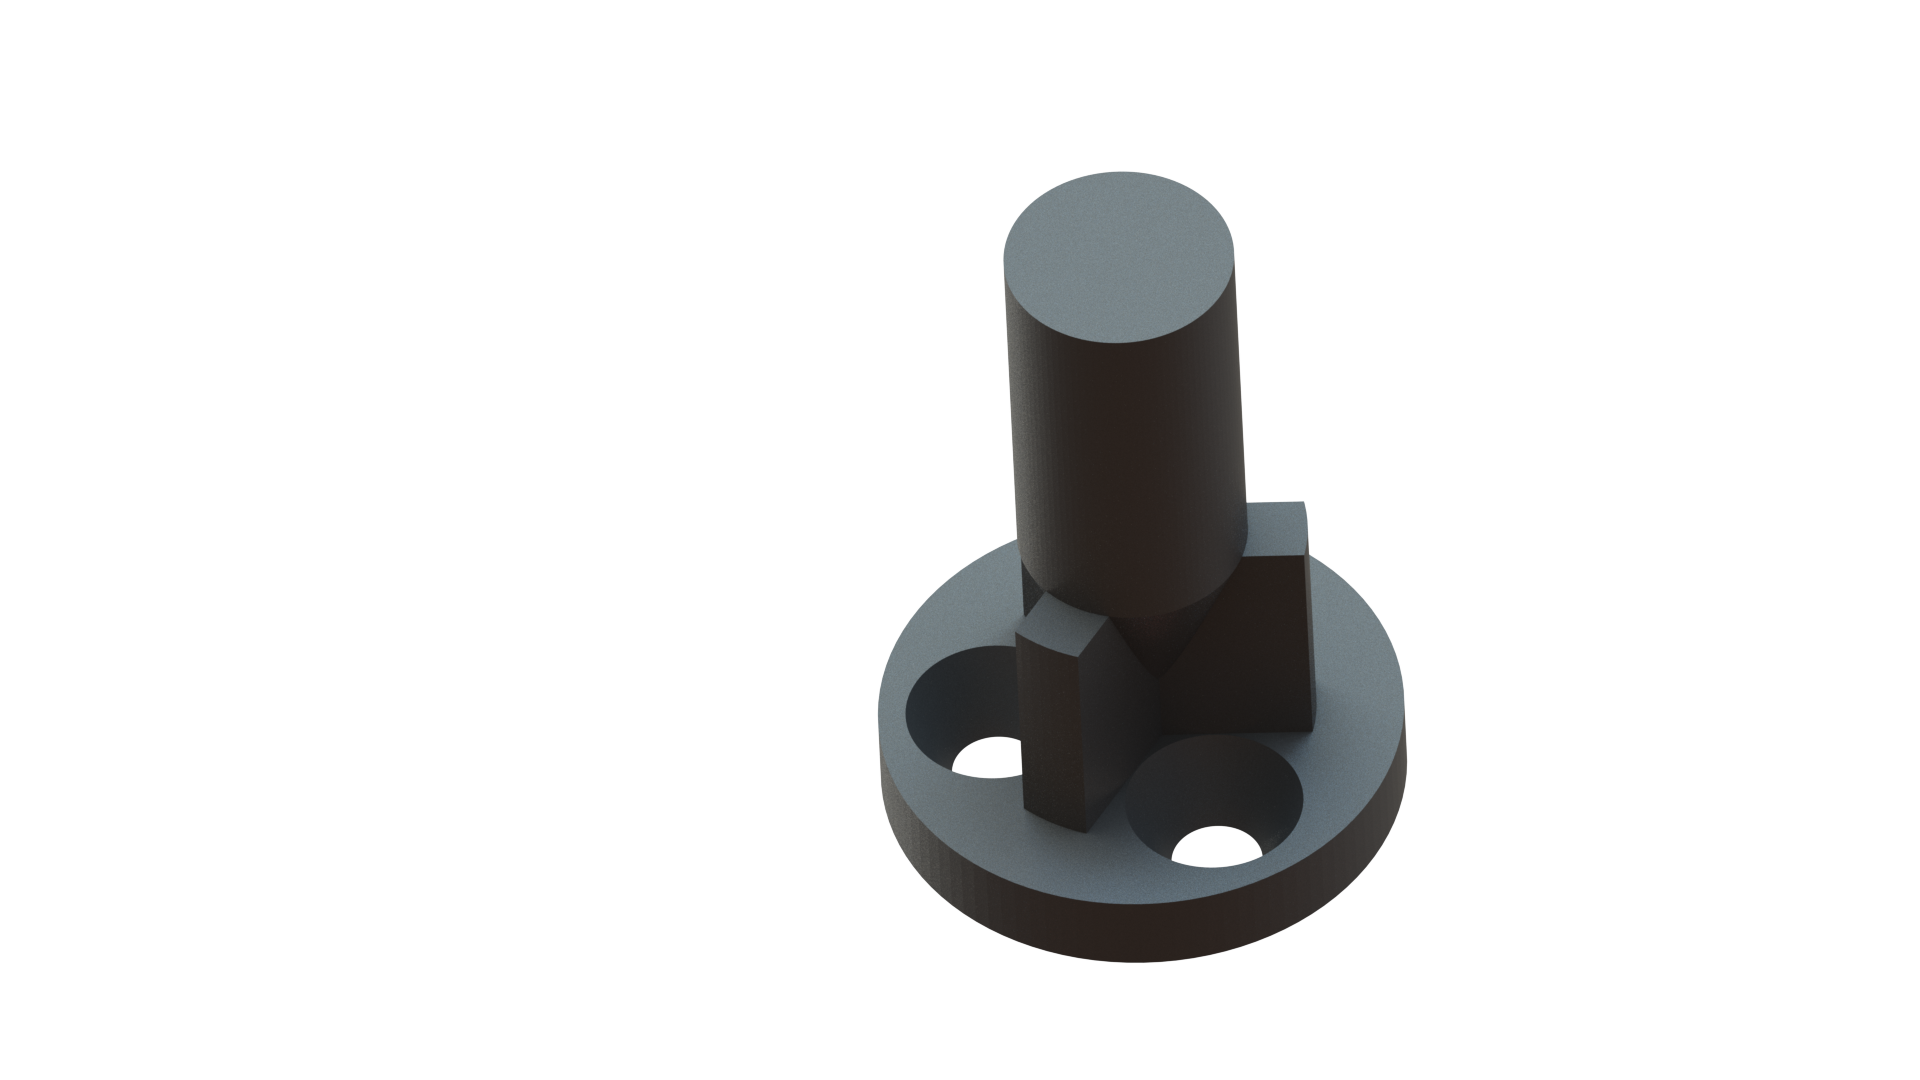
\includegraphics[clip, trim = 6cm 1cm 3cm 1cm, width=0.4\textwidth]{images/mechanical/encoder-shaft} 
\caption{3D printed PLA motor encoder shaft.}
\label{fig:encoder-shaft}
\end{figure} 

\subsection{Tuning and Optimisation}

\definecolor{smokyblack}{rgb}{0.06, 0.05, 0.03}
\chapter{Communication Protocol}

\section{FreeRTOS}

Ideally FreeRTOS tasks should operate with as much isolation as possible, with each task performing a specific function with different priority levels. In the case of a communication protocol, the overall task is inherently sequential so this leads to FreeRTOS being used in a sequential way with all tasks operating at real-time priority level. 

FreeRTOS was chosen because of the following benefits:

\begin{enumerate}
\item Segmentation of code into specific tasks provides readable code for future users.
\item FreeRTOS task configuration provides a framework for future embedded robotic control systems as well as easily reconfigurable code.
\item Semaphores and queues lend themselves to sequential reception and processing of packets at predefined intervals very well.
\item Isolation of tasks provides easy debugging of communication issues.
\end{enumerate}

\subsection{Heartbeat Task}
\subsection{PC TX Task}
\subsection{PC RX Task}
\subsection{TX Motor Task}
\subsection{RX Motor Task}
\subsection{Controller Task}

\subsection{FreeRTOS Timing}

The default 1000 Hz tick rate was overridden with a tick rate of 5000 Hz to enable more fine tuned packet timing and delays. The timing configuration can be seen in \cref{listing:FreeRTOS timing}. 

In order to achieve a control loop rate of 200 Hz, a sampling time of 5 ms or 25 ticks was used.

\section{Packet Encoding and Decoding}

SeqBits bits 2-5 switch case

\begin{figure}
\centering
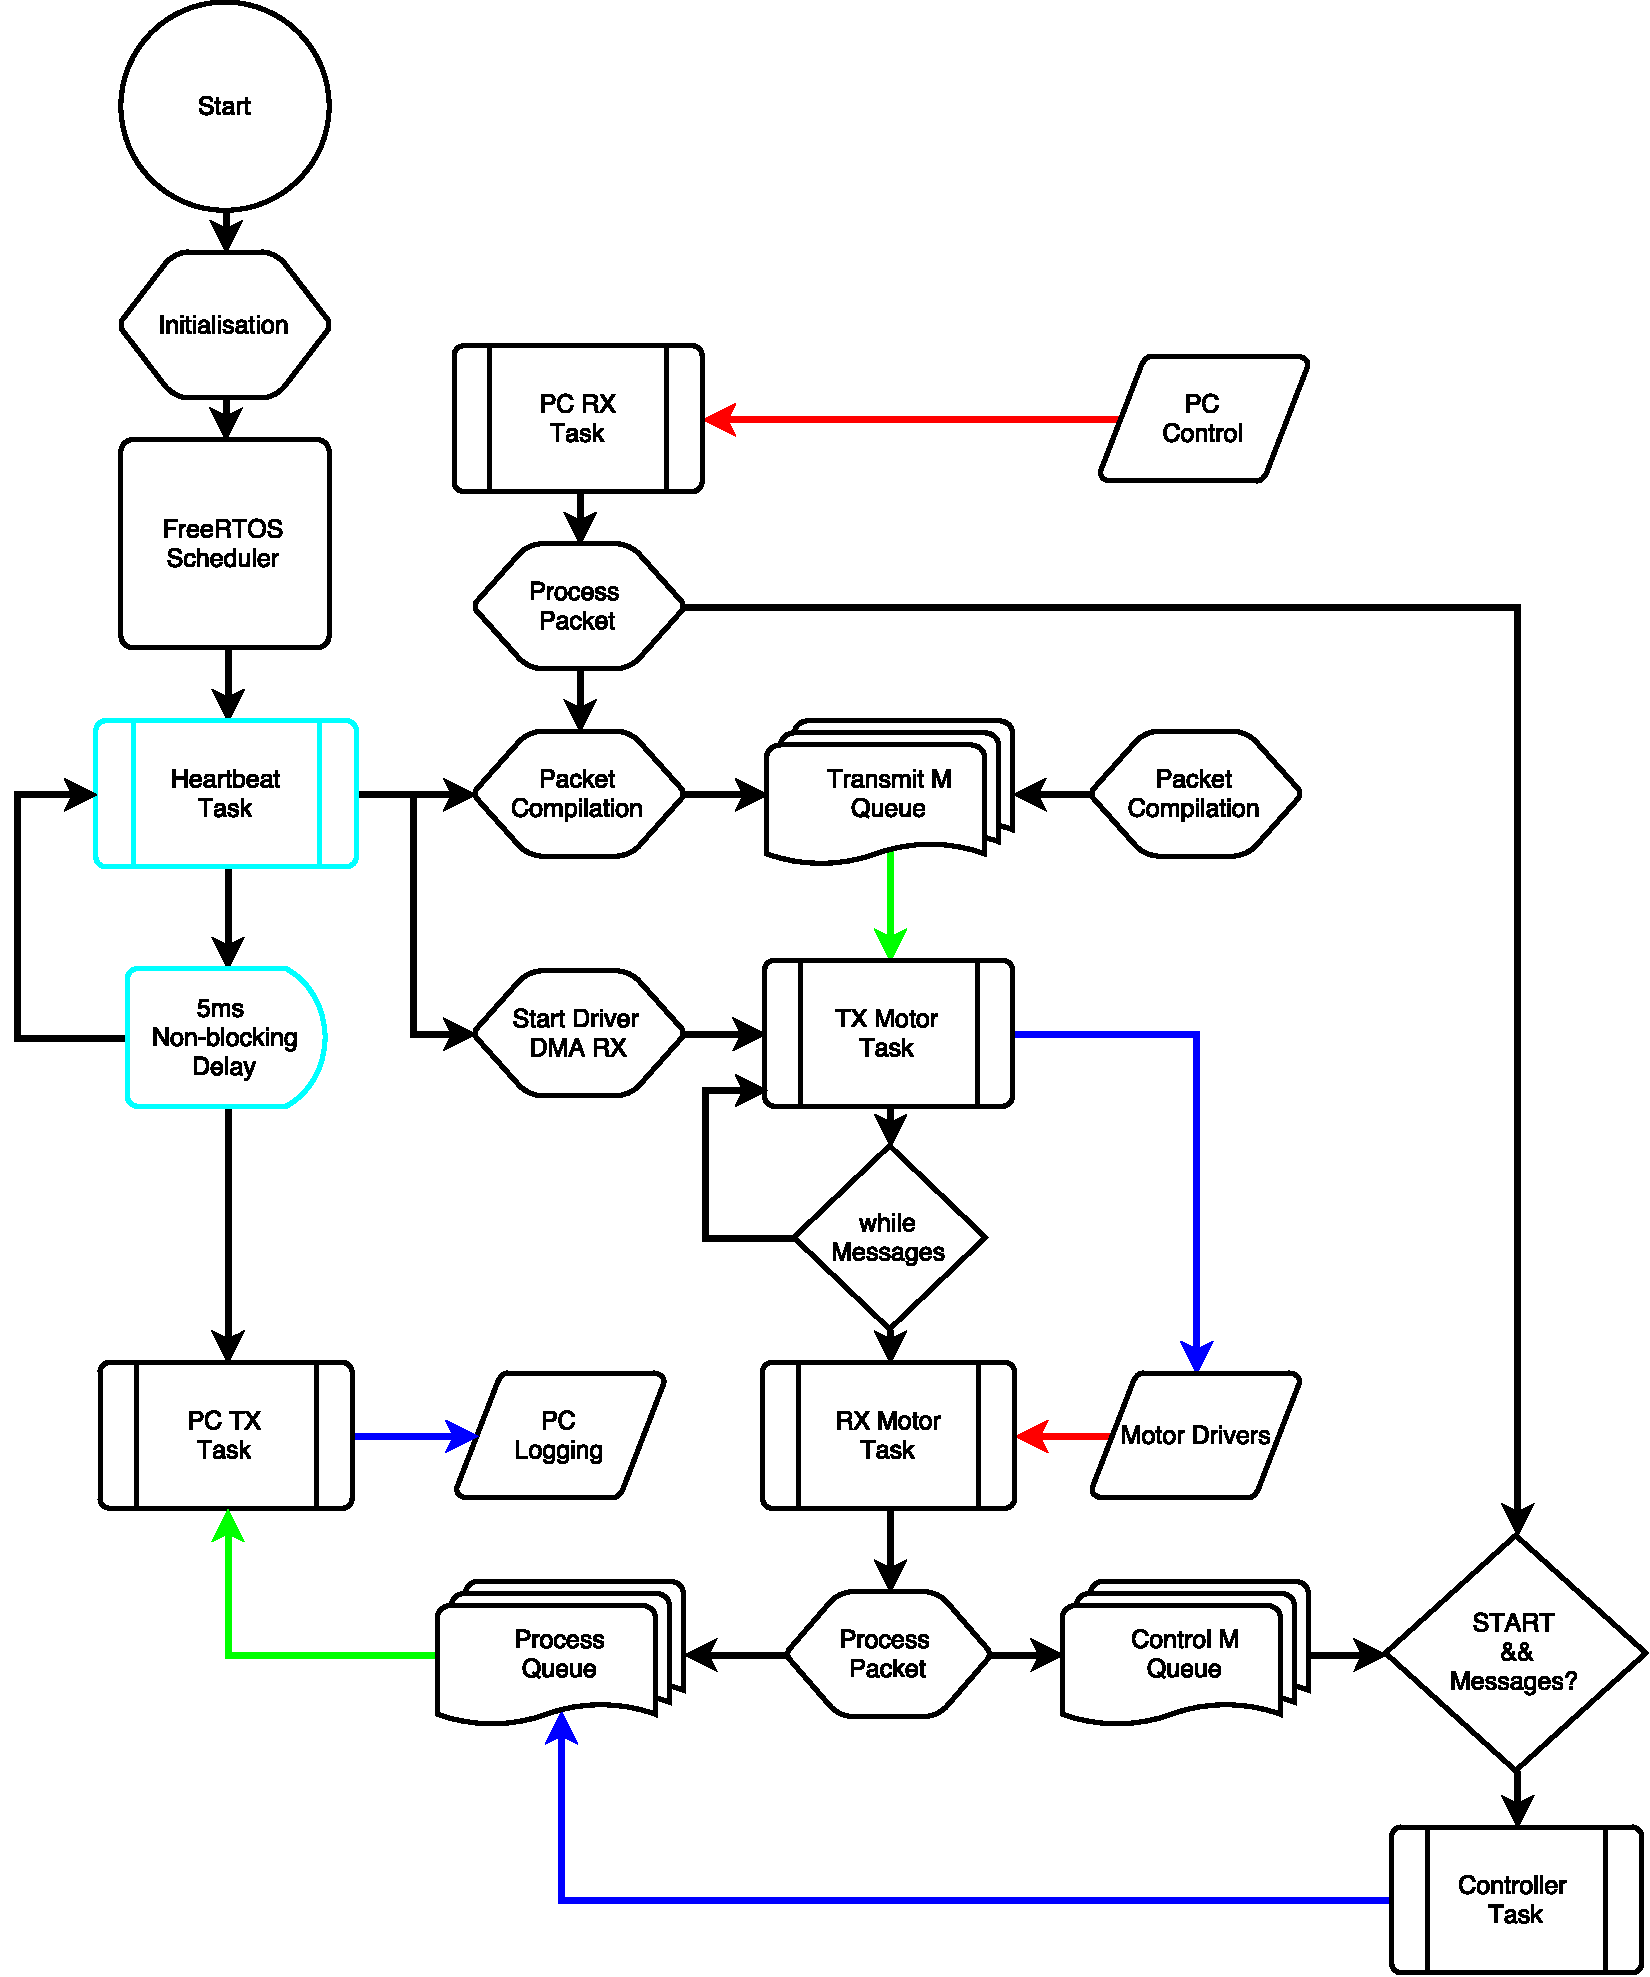
\includegraphics[width=1\textwidth]{images/comms/communication-flow-diagram.pdf} 
\caption{FreeRTOS communication protocol flow diagram.}
\label{fig:FreeRTOS communication protocol flow diagram.}
\end{figure}

\begin{figure}
\centering
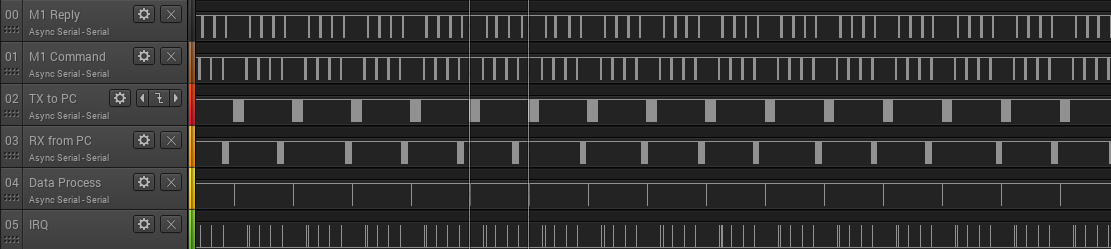
\includegraphics[width=1\textwidth]{images/comms/pc-packet-timing-data} 
\caption{Communication protocol packet timing with 5 ms sampling rate.}
\label{fig:packet-timing.}
\end{figure}

\begin{table}
\centering
\begin{tabular}{llllll}
\textbf{Command}       & \textbf{Index} & \textbf{Op-Code} & \textbf{TX CB} & \textbf{TX CRC1} & \textbf{RX  CB} \\
\textbf{Kill Bridge}   & 1              & 0001             & 0x06           & 0xCBB6           & 0x04            \\
\textbf{Write Enable}  & 2              & 0010             & 0x0A           & 0x3624           & 0x08            \\
\textbf{Bridge Enable} & 3              & 0100             & 0x12           & 0x1AE0           & 0x10            \\
\textbf{Set Current}   & 4              & 0011             & 0x0E           & 0xBF7B           & 0x0C            \\
\textbf{Read Current}  & 5              & 1100             & 0x31           & 0x9772           & 0x32            \\
\textbf{Read Position} & 6              & 1111             & 0x3D           & 0xD310           & 0x3E            \\
\textbf{Read Velocity} & 7              & 0101             & 0x15           & 0x5EAF           & 0x16            \\
\textbf{Set Position}  & 8              & 1010             & 0x2A           & 0x42C4           & 0x28           
\end{tabular}
\caption{Motor driver command protocol.}
\label{tab:motor-driver-protocol}
\end{table}
%\chapter{Graphic User Interface}

\section{Serial Communication}

\begin{figure}
\centering
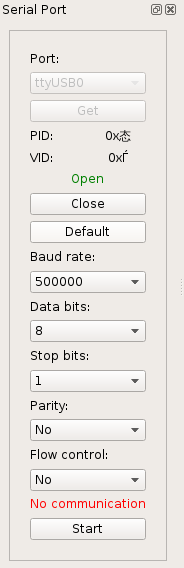
\includegraphics[width=0.3\textwidth]{images/gui/serial-port}
\end{figure}

\section{Logging}

\begin{figure}
\centering
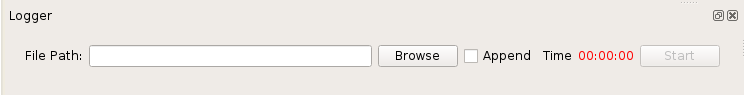
\includegraphics[width=0.8\textwidth]{images/gui/logger}
\end{figure}

\section{Live Plotting}

\begin{figure}
\centering
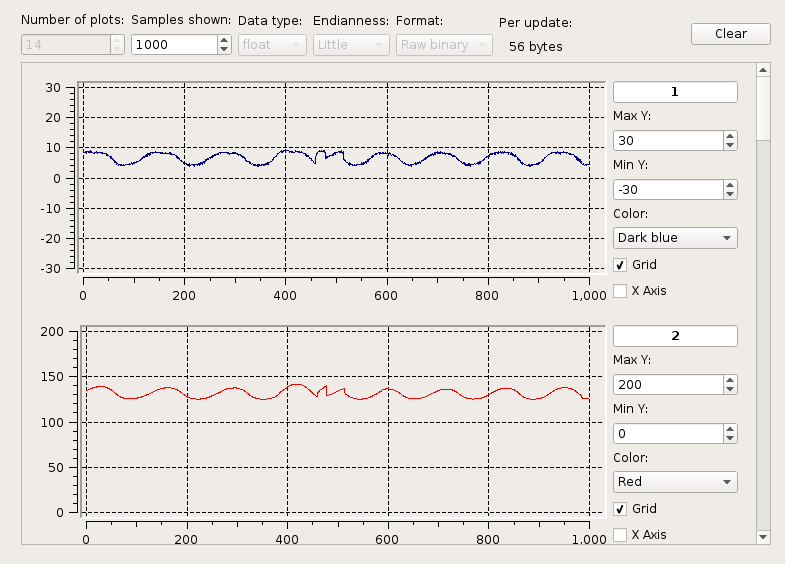
\includegraphics[width=0.7\textwidth]{images/gui/plotting}
\end{figure}

\section{Control Plug-in}

\begin{figure}
\centering
\subfloat[][Configuration \& On-board Control]{
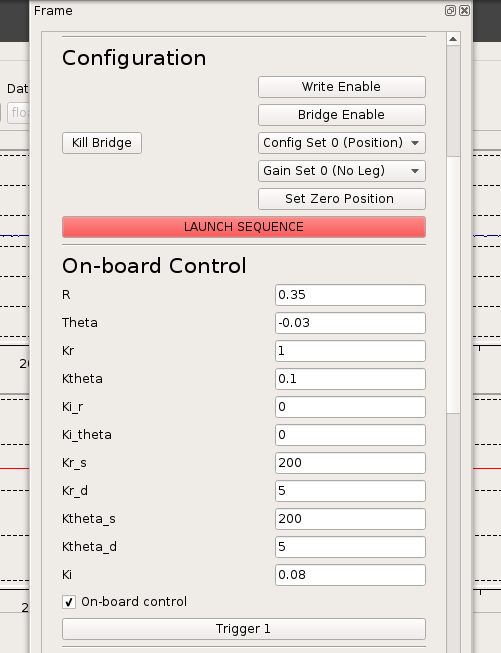
\includegraphics[width=0.4\textwidth]{images/gui/frame-1}
}
~
\subfloat[][Current/Position Control \& Control Loop Gains]{
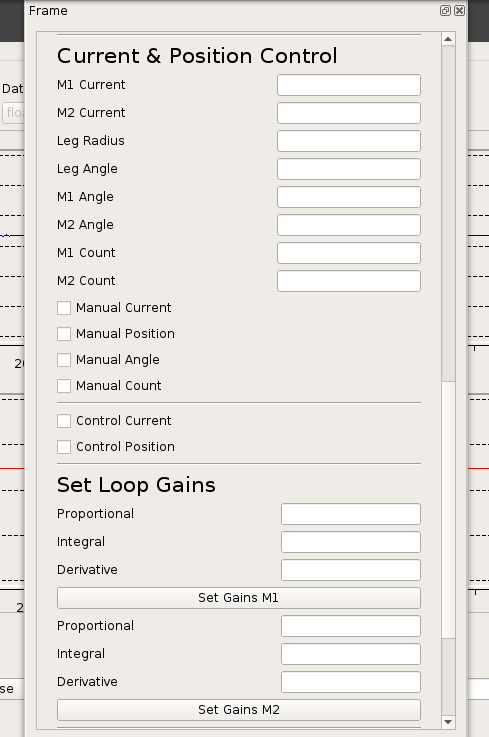
\includegraphics[width=0.4\textwidth]{images/gui/frame-2}
}
\caption{Control interface plug-in.}
\label{fig:Control interface plug-in} 
\end{figure}


\chapter{Dynamic Modelling}
\section{System Modelling}

\begin{figure}
\centering
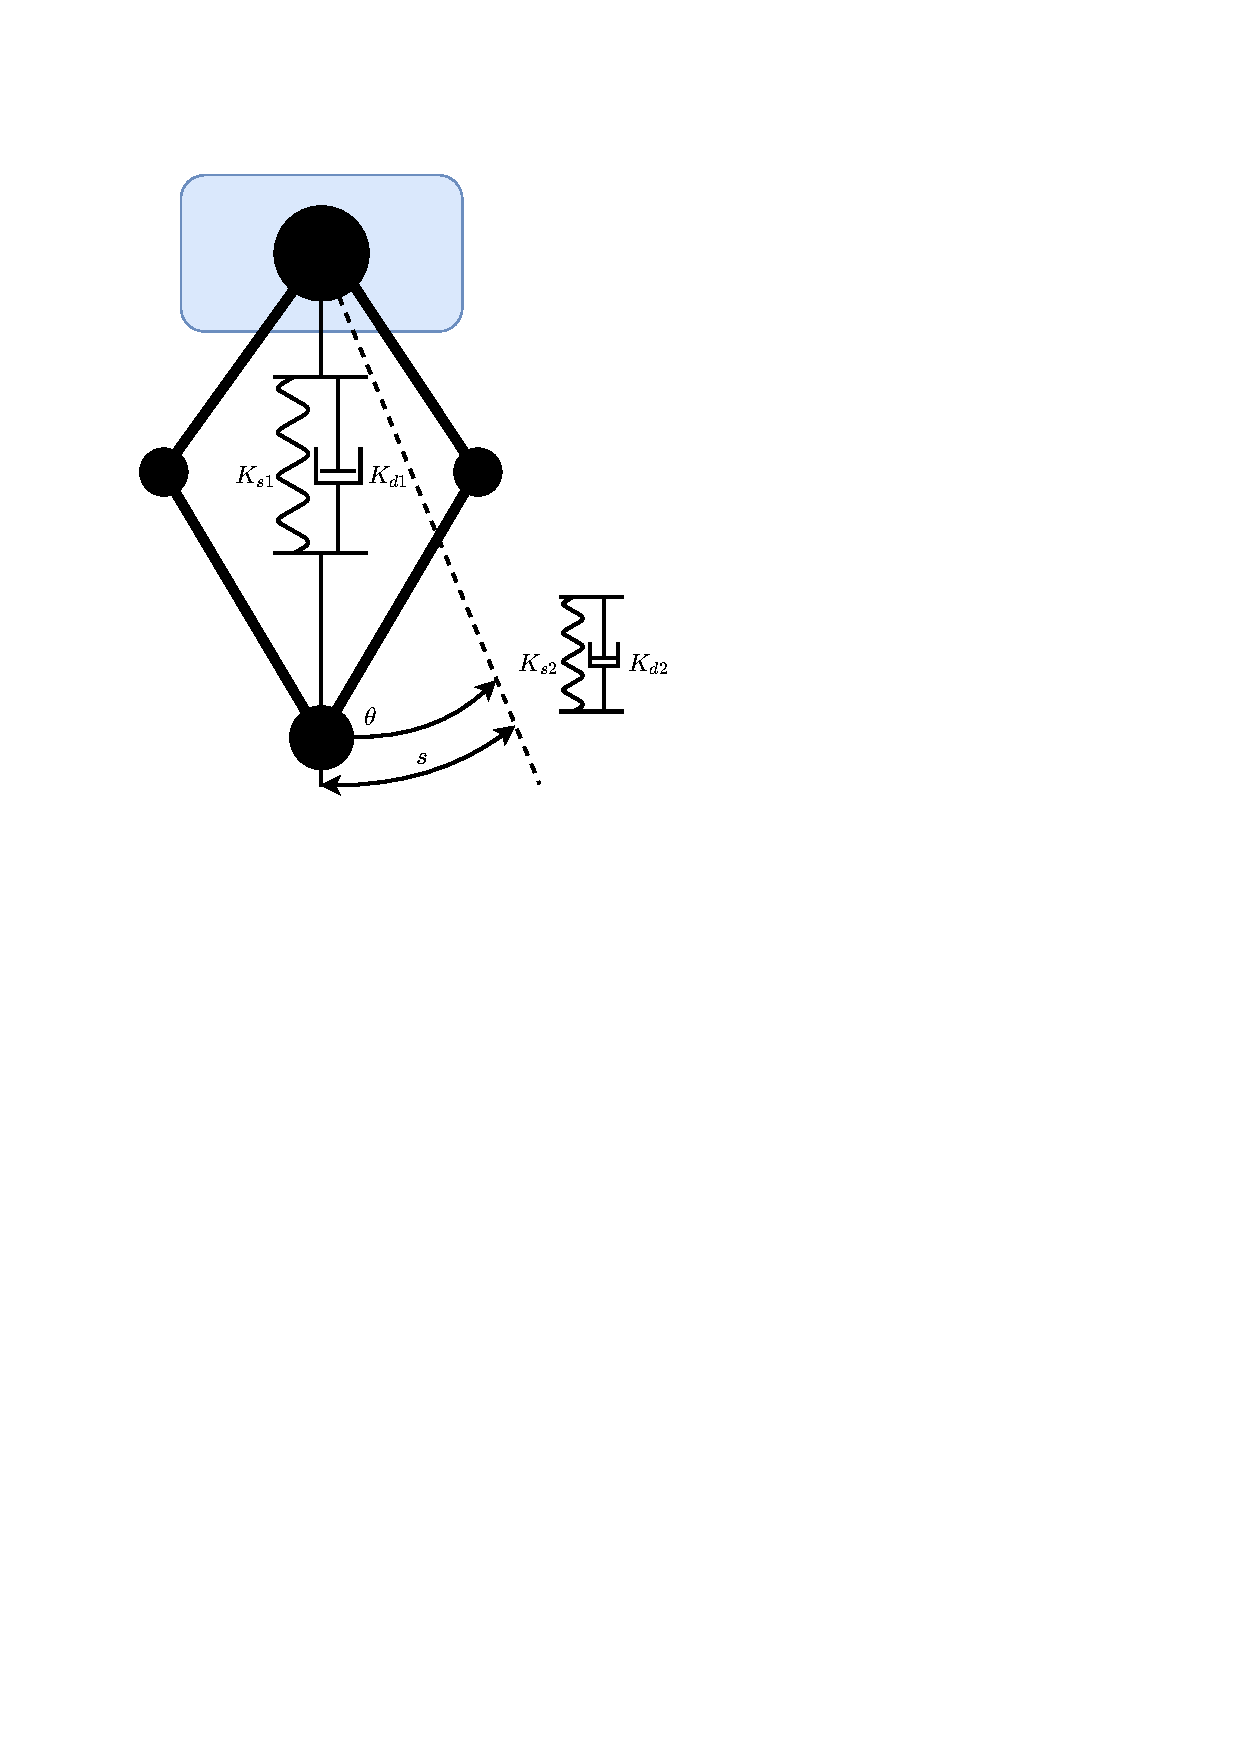
\includegraphics[clip, trim=2cm 15cm 9cm 2cm, page = 1, width=0.8\textwidth]{images/geometry/leg-spring-damper} 
\caption{Leg spring-damper virtual model.}
\label{fig:Leg spring-damper virtual model}
\end{figure}

\subsection{SLIP Model}
\section{Virtual Compliance Model}
\chapter{Controller Development}

\section{Dynamic Actuation}


\setchapterpreamble[uc][.75\textwidth]{%
\dictum[Van Halen, \textit{1984}]{%
``Jump!''}\vskip1em}

\chapter{Experimental Testing}

$r_0 = 0.3\ m$\\
$r_{offset} = r - r_0 = 0.13\ m$

\begin{figure}
\centering
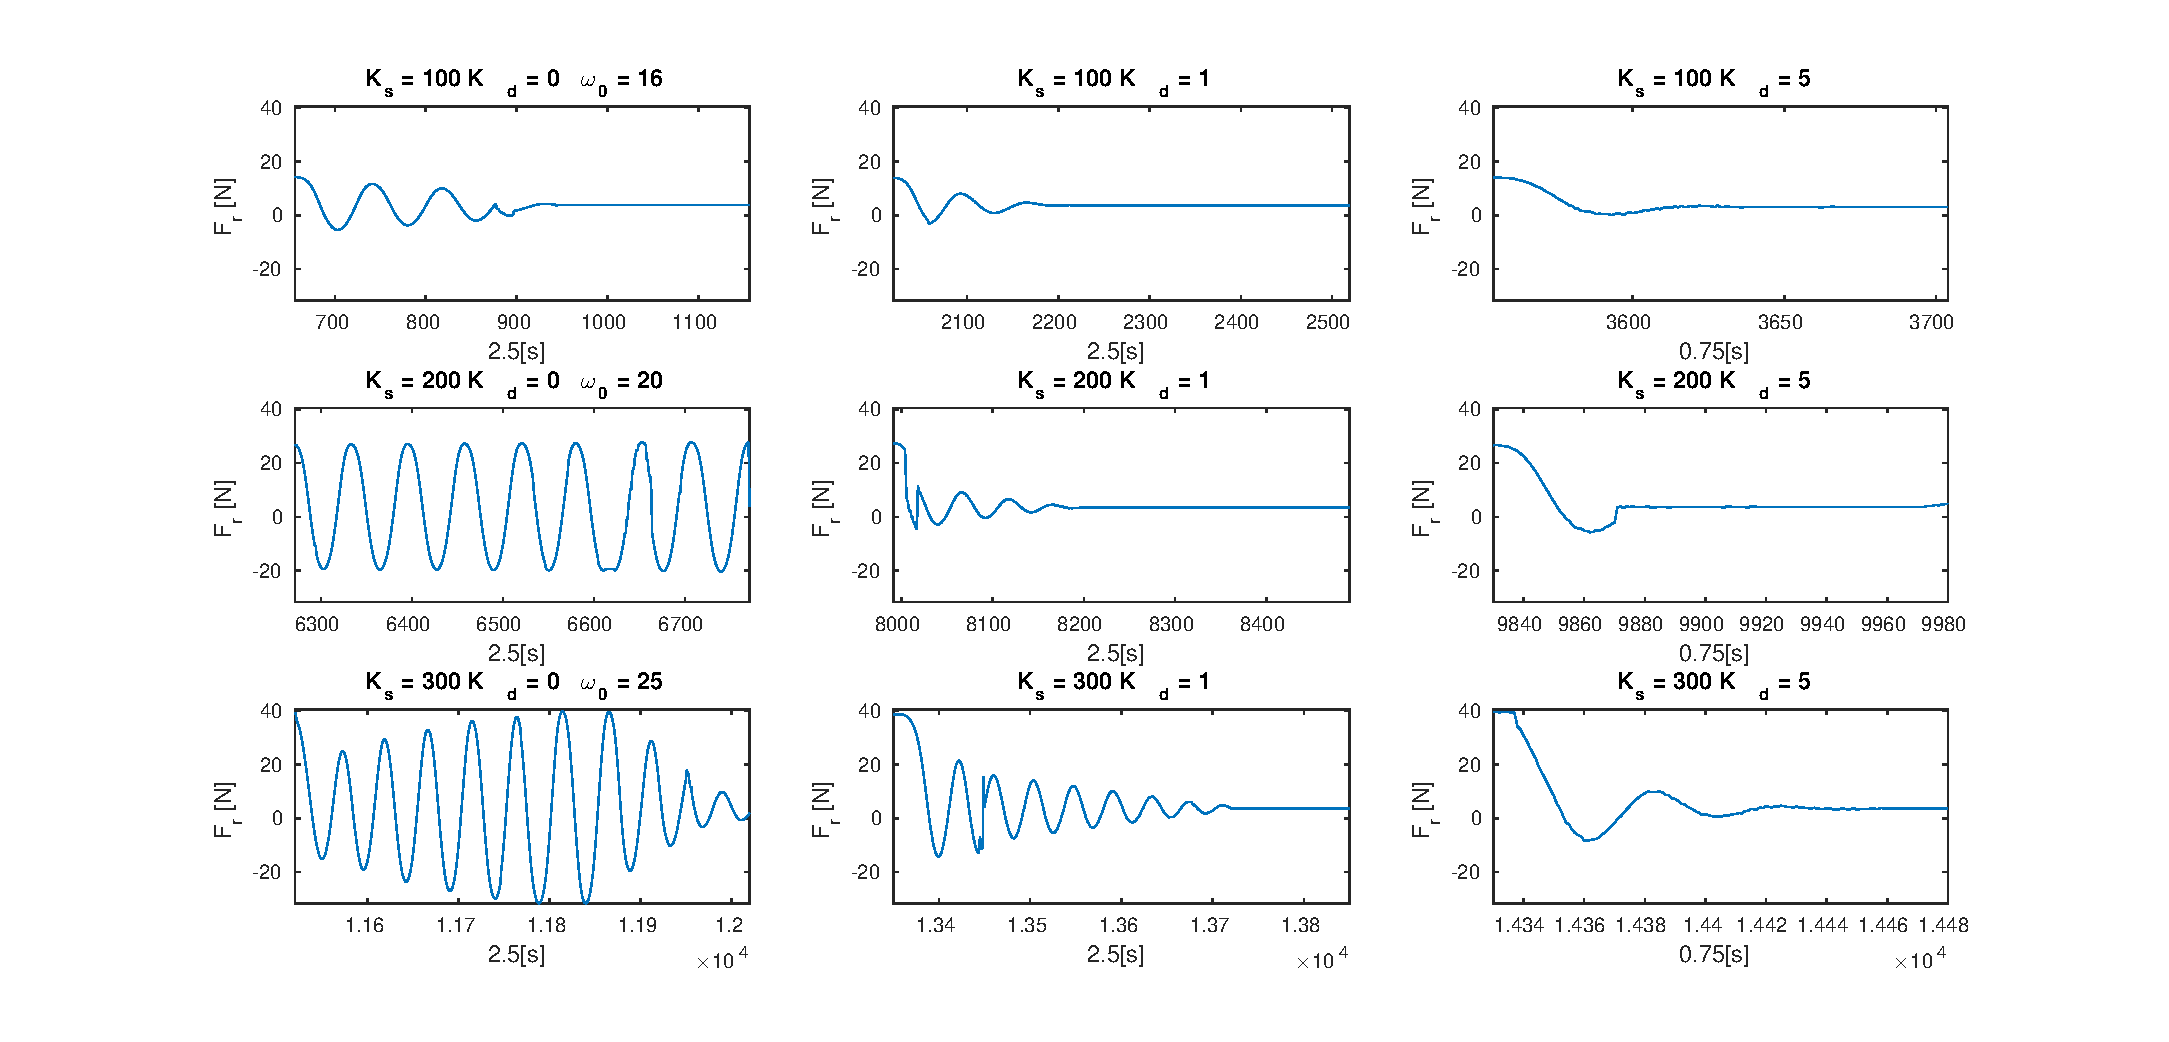
\includegraphics[width=1\textwidth]{images/logging/spring-damper-tests.eps} 
\caption{Leg spring damper testing for radial offset.}
\label{fig:spring-damper-tests}
\end{figure}
\chapter{Design Validation}
\chapter{Conclusions}
\chapter{Recommendations and Future Work}
\lipsum

%\bibliographystyle{ieeetran}
\renewcommand{\bibname}{References}
\bibliography{aux/bibliography}
\bibliographystyle{ieeetran}
\renewcommand{\bibname}{References}
\bibliography{aux/bibliography}

\appendix
\chapter{Code}
\lipsum
\chapter{Workspace Data}

Research data is separated into the folders as listed below, available on CD or by request:

\begin{itemize}
\item background: various literature review documents.
\item baleka-stm32f4-code: embedded system code.
\item BalekaQtApp: Qt GUI code.
\item baleka-system-kicad: start of electronics CAD representation of embedded system.
\item communication: embedded system and motor driver communication protocol work.
\item datasheets: various datasheets of components used in leg design.
\item documentation: start of documentation write-up for Driveware use and configuration.
\item drawio: draw.io graphic design application files used for report.
\item experiments: experimental test data and video data.
\item kinematics: various files with kinematic constraints and motor driver position limits.
\item LATEX: report write-up in LATEX.
\item miscellaneous: mass logs, motor model tuning, and performance tables.
\item solidworks-original: compressed folder of all Ben Bingham's original CAD work.
\item VacWorkLeg-original: compressed folder of all Luke Bell's original work.
\item workspace-atollic: initial development of embedded system code.
\item workspace-driveware: Driveware motor driver configuration files.
\item workspace-inemo: work completed on iNemo code developed by Callen Fisher.
\item workspace-matlab: Matlab scripts and saved workspaces.
\item workspace-openscad: OpenSCAD programmatic CAD models.
\item workspace-solidworks: CAD assemblies, designs and virtual models developed in Solidworks.
\end{itemize}

The final report write-up PDF can be found in the root directory, named report.pdf.
\chapter{Jump Experiment}
\label{app:Jump Experiment}

\begin{table}[!ht]
\centering
\begin{tabular}{l|llll}
\textbf{Frame (no.)} & \textbf{Time (ms)} & \textbf{Height (m)} & \textbf{Interval Velocity (m/s)} & \textbf{Phase}\\
0	&	0	&	0.00000	&	0.000	&	Stance	\\
1	&	84	&	0.05000	&	0.595	&	Decompression launch	\\
2	&	126	&	0.12500	&	1.786	&	Decompression launch	\\
3	&	167	&	0.21250	&	2.134	&	Flight	\\	
4	&	209	&	0.25000	&	0.893	&	Flight + Recovery	\\
5	&	292	&	0.29375	&	0.527	&	Flight + Recovery	\\
6	&	376	&	0.26250	&	-0.372	&	Freefall	\\
7	&	501	&	0.12500	&	-1.100	&	Freefall	\\
8	&	543	&	0.07500	&	-1.190	&	Impact	\\
9	&	584	&	0.00000	&	-1.829	&	Compliant landing	\\
10	&	709	&	0.02500	&	0.200	&	Compliant landing	\\
11	&	793	&	0.04375	&	0.223	&	Compliant landing
\end{tabular}
\caption{Launch and compliant landing video frame data.}
\label{tab:jump-test-data}
\end{table}

\begin{figure}
\centering
\subfloat[][Frame 0.]{
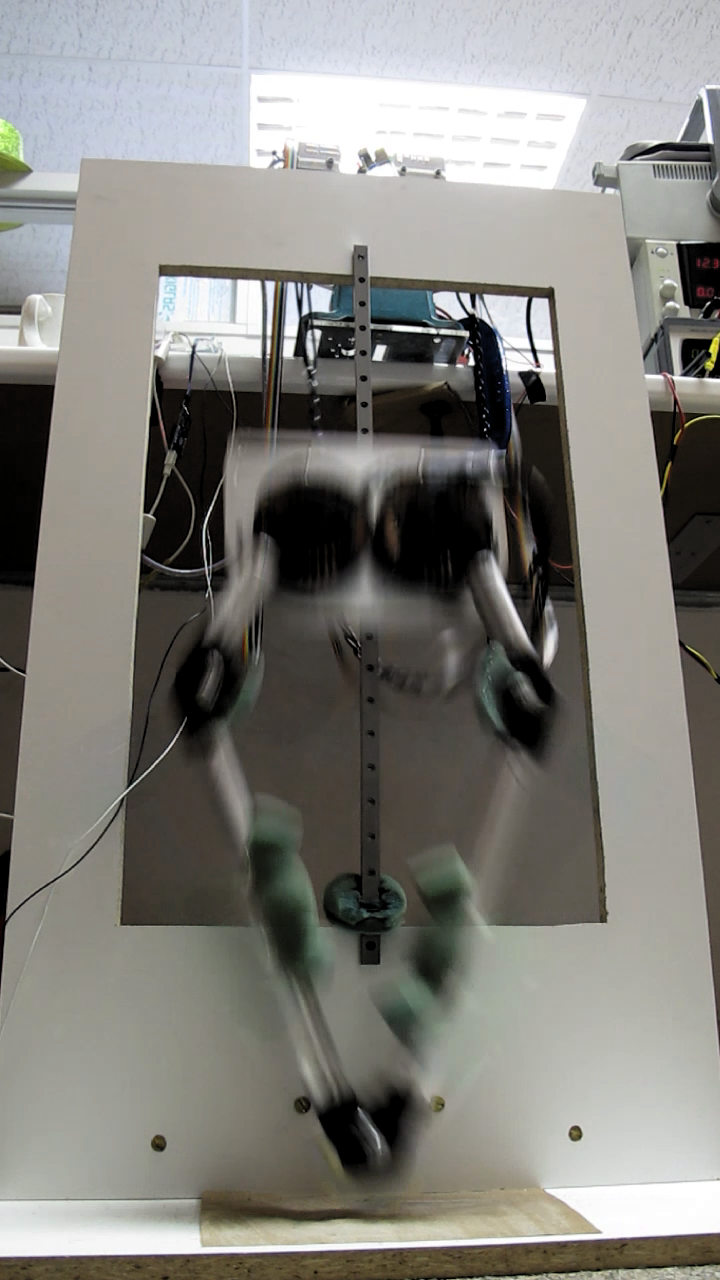
\includegraphics[width=0.3\textwidth]{images/experiments/failed-jump/0.png} 
}
~
\subfloat[][Frame 1: Current cut-out.]{
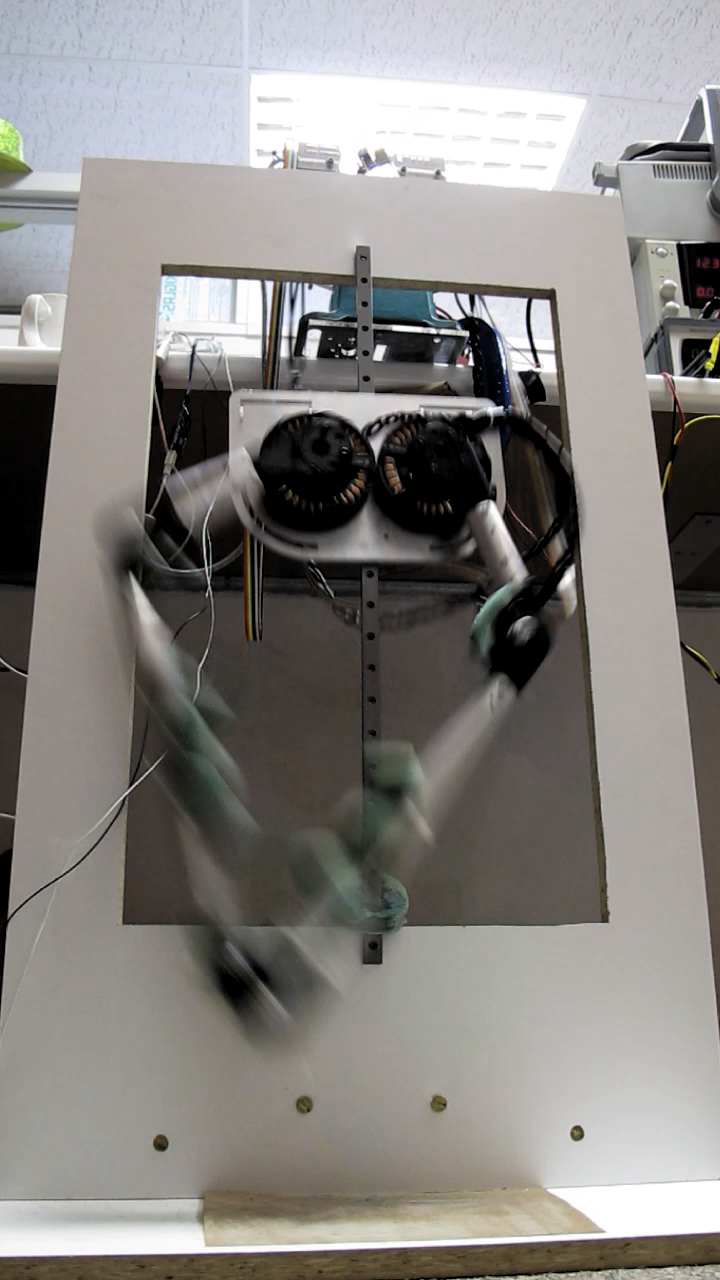
\includegraphics[width=0.3\textwidth]{images/experiments/failed-jump/1.png} 
}
~
\subfloat[][Frame 2.]{
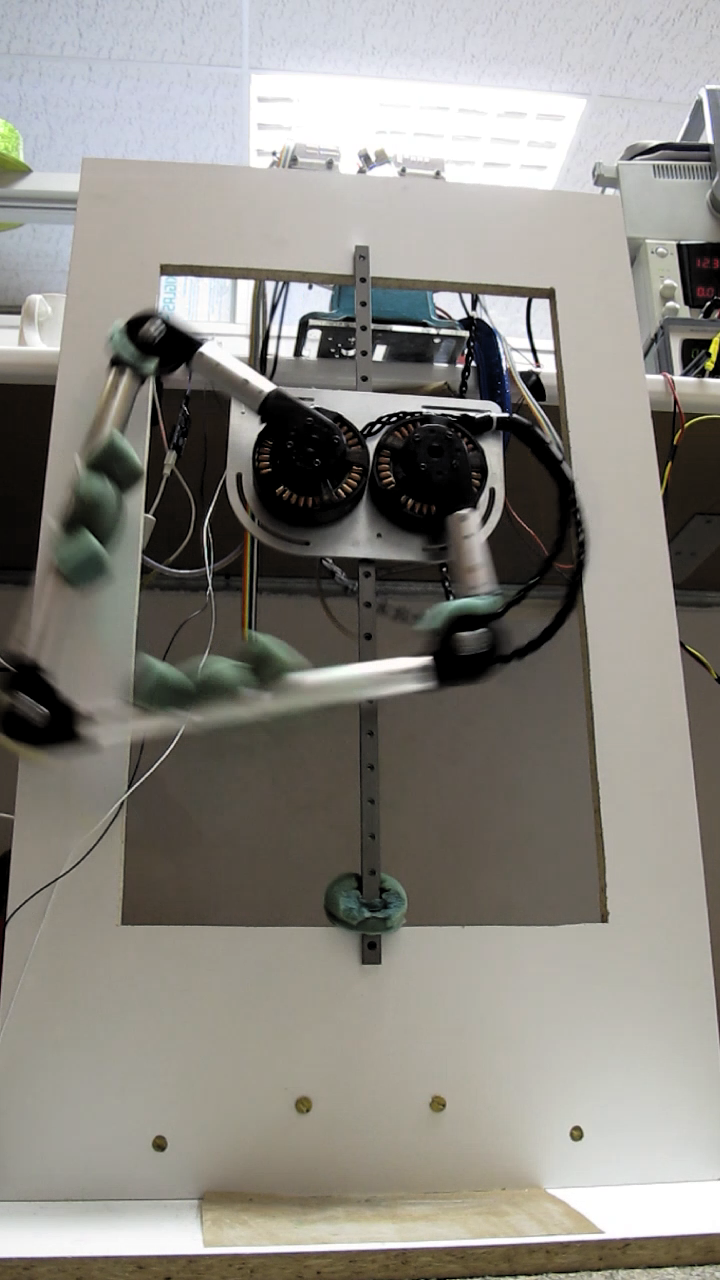
\includegraphics[width=0.3\textwidth]{images/experiments/failed-jump/2.png} 
}

\subfloat[][Frame 3.]{
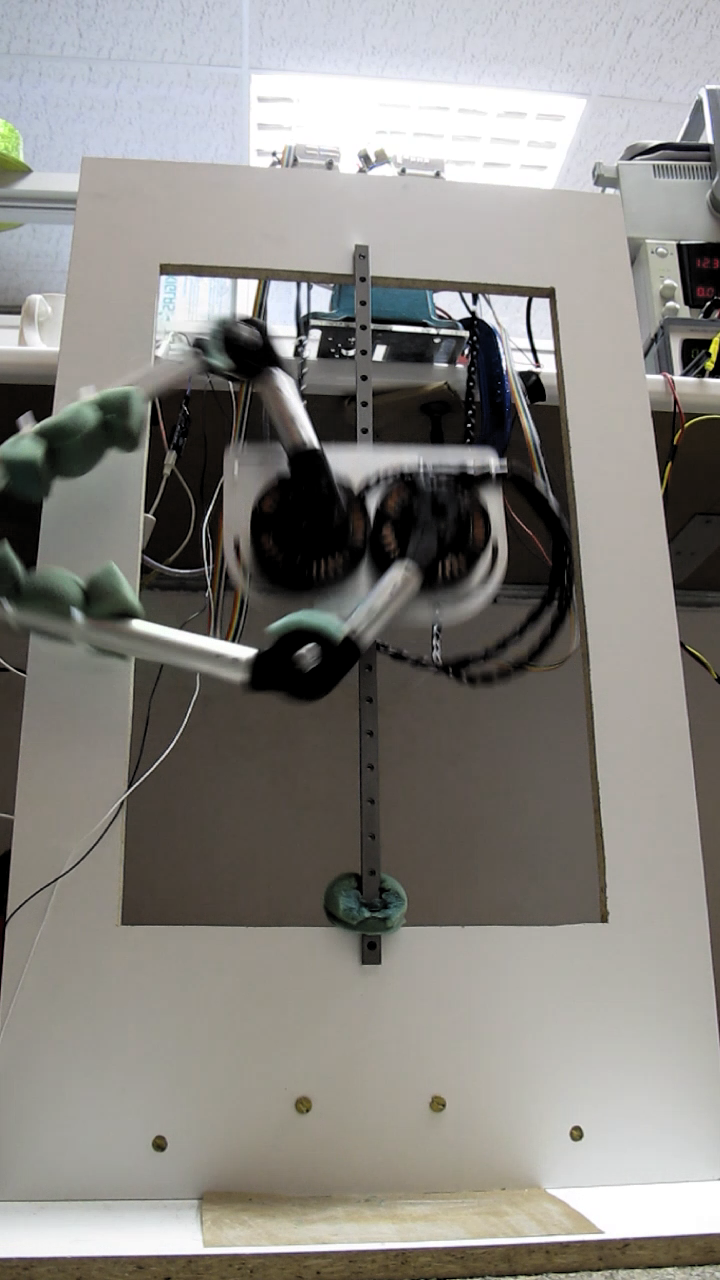
\includegraphics[width=0.3\textwidth]{images/experiments/failed-jump/3.png} 
}
~
\subfloat[][Frame 4.]{
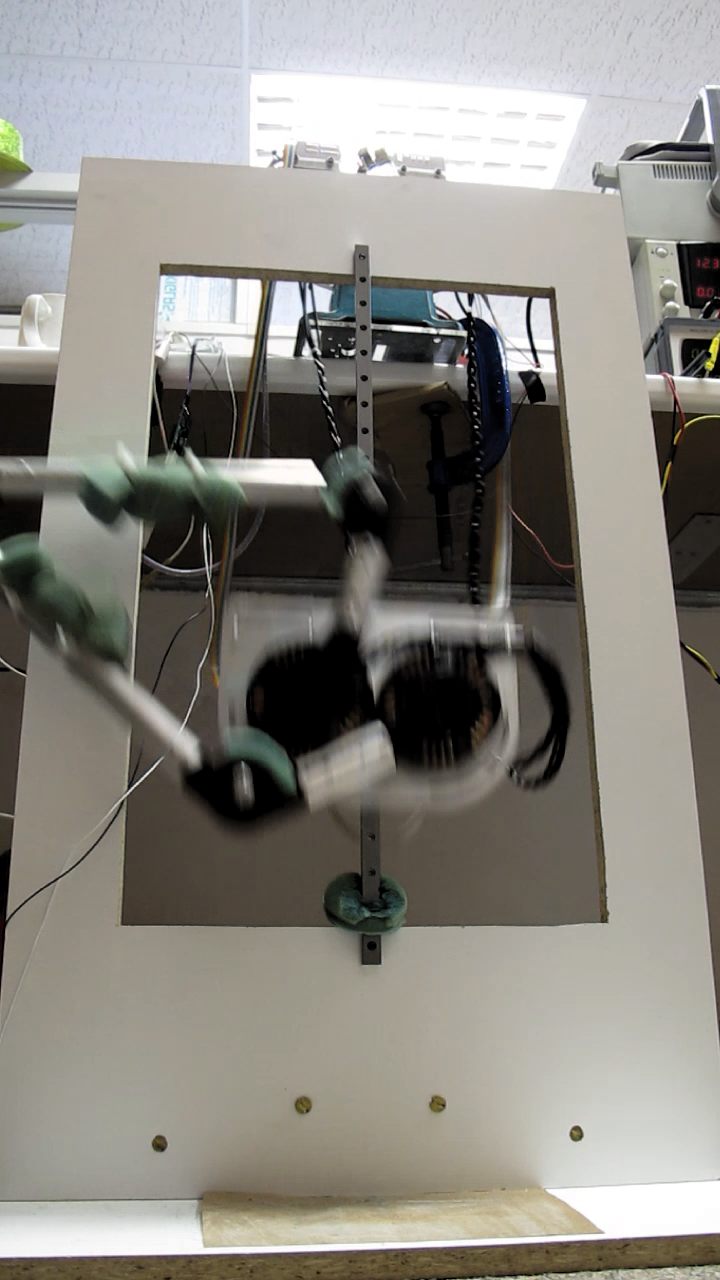
\includegraphics[width=0.3\textwidth]{images/experiments/failed-jump/4.png} 
}
~
\subfloat[][Frame 5.]{
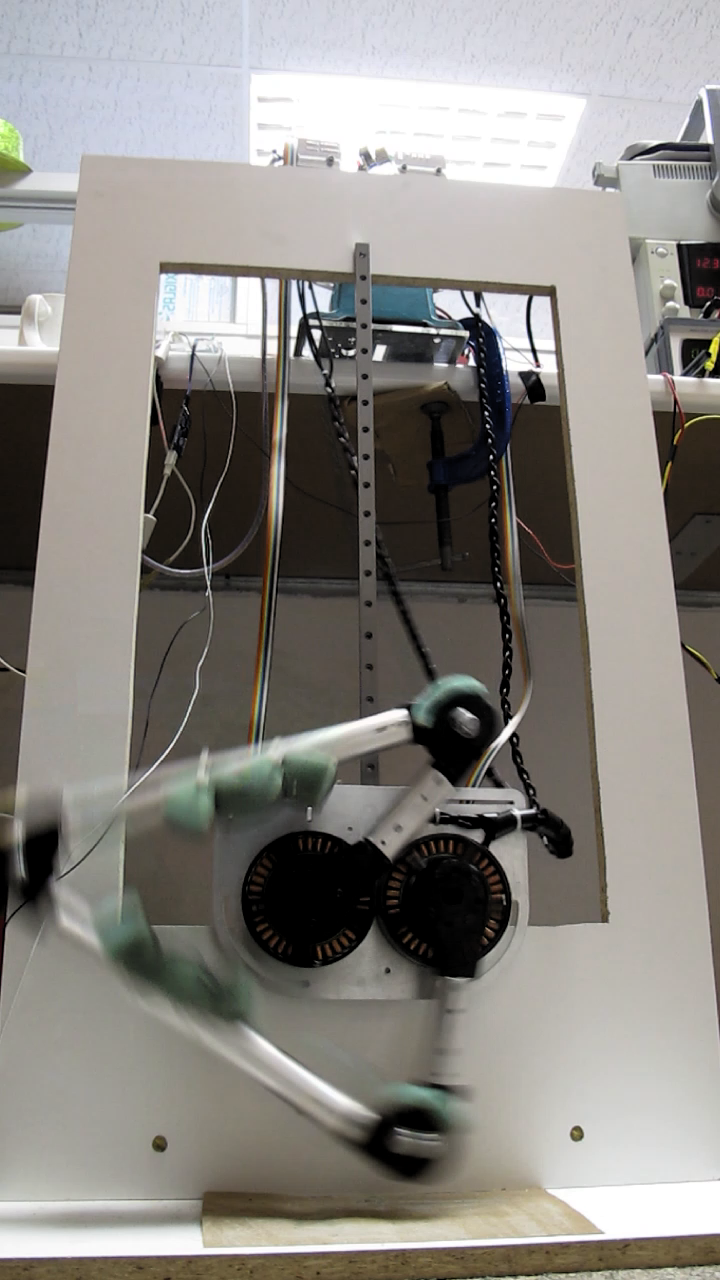
\includegraphics[width=0.3\textwidth]{images/experiments/failed-jump/5.png} 
}
\caption{Motor driver over-current cut-out.}
\label{fig:Motor driver over-current cut-out}
\end{figure}

\begin{listing}[ht]
\begin{minted}[
linenos,
bgcolor=smokyblack]{c}
if(SHOT && r_fbk >= 0.38) {
        r_cmd = 0.3;
        k_r = 1;
        k_s = 0.1;
        ks_r = 633;
        kd_r = 15;
        ks_s = 400;
        kd_s = 5;
        SHOT = 0;
        TRIGGER = 1; //DANGEROUS!
}
if(PULLED && (ELAPSED > 1000)) {
        r_cmd = 0.4;
        k_r = 1;
        k_s = 0.1;
        ks_r = 1726;
        kd_r = 0;
        ks_s = 400;
        kd_s = 5;
        SHOT = 1;
        PULLED = 0;
        ELAPSED = 0;
}
if(TRIGGER) {
        r_cmd = 0.25;
        k_r = 1;
        k_s = 0.1;
        ks_r = 633;
        kd_r = 15;
        ks_s = 400;
        kd_s = 5;
        ELAPSED = 0;
        TRIGGER = 0;
        PULLED = 1;
}
else{
        ELAPSED++;
}
\end{minted}
\caption{Jump control condition loop.}
\label{listing:Jump control condition loop}
\end{listing}
\chapter{Geometric Simulation Code}

\begin{listing}[ht]
\begin{minted}[
linenos,
bgcolor=smokyblack]{Matlab}
l1 = 0.15; %length of upper linkage in m (measured from center of joint of 5 cm diameter)
l2 = 0.3; %length of lower linkage in m (measured from center of joint of 5 cm diameter)

phi1 = (1/9*pi):0.125:pi; % all possible phi1 values
phi2 = (1/9*pi):0.125:pi; % all possible phi2 values

[PHI1, PHI2] = meshgrid(phi1, phi2); % generate a grid of phi1 and phi2 values

R = -l1*cos((PHI1 + PHI2)./2) + sqrt(l2^2 - l1^2*sin((PHI1 + PHI2)./2).^2);
THETA = (PHI1 - PHI2)./2;

plot(THETA(:), R(:), 'r.', 'MarkerSize', 20);
\end{minted}
\caption{Geometric simulation code to generate kinematic workspace.}
\label{listing:Geometric simulation code}
\end{listing}

\end{document}
